\documentclass{article}

\usepackage[utf8]{inputenc}
\usepackage[left=1.5in,right=1.5in,bottom=1in]{geometry}
\setlength\parindent{0pt}
\setlength{\parskip}{1em}
\setcounter{secnumdepth}{0}
\usepackage{outlines}
\usepackage{graphicx}
\graphicspath{ {imgs} }
\usepackage{hyperref}

\title{Urban Economic Geography}
\author{Carla Hyenne }

\begin{document}

\maketitle

\tableofcontents

\pagebreak

%%%%%%%%%%%%%%%%%%%%%%%%%%%%%%%%%%%%%%%%%%%%%%%%%%%%%%%%%%%
% 																		 LECTURE 1
%%%%%%%%%%%%%%%%%%%%%%%%%%%%%%%%%%%%%%%%%%%%%%%%%%%%%%%%%%%

\section{The City as a Social Product}
\date{September 30th, 2021}

There is no such thing as a "pure", "neutral" knowledge or definition of cities/urban space. There are empirical observations, like the density, retail, urban projects, transport, road safety regulations, etc. However, what we see isn't enough. We need concepts, theories, models, abstract tools to make sense of the city.

The type of "intellectual" glasses that we wear influence what and how we understand the space and the issues within it. For example in economics, your views change if you are wearing capitalist vs. socialist glasses.

Thus, what epistemological choices is this class based on? It takes distance from the "urban triumphalism" mainstream, and takes a critical stance on urban issues. 

\subsection{Urban Triumphalism}

Triumphalism depicts cities as a site of progress, a way to prosperity, and we are in a "golden age" of the city. The major \textbf{contemporary challenges} are first urban challenges, and the urban space is where \textbf{solutions} are found. Think of the green, smart, productive, participative, etc., city. 

The key question is then \textit{how} to re-organise the city in order to meet these challenges, by using the potentialities and opportunities in the urban environment. 

\subsubsection{What is the problem with urban triumphalism?}

\begin{outline}
  \1 Urban triumphalism is purely a pro-growth perspective, which is contradictory with the sustainability targets (continuous growth is not sustainable). 
  \1 It is only about finding solutions to a series of pre-defined challenges: how to build the city, equip the city, govern the city, brand the city... This turns urban issues into \textbf{techno-management} issues, where the focus in on the best practices that can be copy/pasted, and where the focus is: 
  	\2 on city leaders' views, 
	\2 on best practices for copy/pasting solutions, and 
  	\2 on mass production of city rankings which highlight competition

  \1 Consultancy firms (McKinsey) are now targeting the 'CEOs' of cities, that is the mayors, to propose techno-managerial solutions to urban problems. 
These firms are usually focused on maintaining the \textbf{competitiveness} of cities, so that the livelihoods of residents are maintained. This statement from McKinsey is contradictory, since most residents are not involved in making the city competitive, and could be better off if cities were less capitalist.

The mass production of city rankings, also done by consultancy firms, are not transparent. They emphasise the importance of competition amongst cities

  \1 There is a strong inclination towards \textbf{reification} (treating something immaterial, as a material thing). 
  	\2 The social objects are conceived as a mere thing, a coherent and active whole. Cities are viewed as actors
	\2 The city is viewed as an actor ("the city does this"), and acts according to a series of shared interests and aspirations. However, what is good for one is not always good for the other (usually, what's good for businesses/elites is not good for the rest) 
\end{outline}

Marcuse, in \textit{The City as a Perverse Metaphor} explains that seeing the city as an actor excludes a set of the population who does not share the same interests and aspirations. Not all the city is international, competitive, and so on, even if some firms, some people might be. 

\subsubsection{Breaking with Triumphalism}

\begin{outline}
	\1 The city is not an actor, but a \textbf{dynamic space} where actors with different resources, interests, aspirations, interact in diverse ways, from open conflict violence to resistance, mobilisation, collaboration, solidarity
	\1 Urban issues are not all \textbf{techno-managerial} ones, but also \textbf{political}
		\2 Urban space are composed of an established web of social relations, sedimented through history in a specific geographical context
		\2 Urban change is therefore fundamentally conflictual, regarding material forms, norms, regulations, symbolic landscapes... (these are political conflicts, where disagreement and lack of consensus is the default)
		\2 Thus, \textbf{urban landscapes are dynamic and contested landscapes of social power}\footnote{Example: the Berlin referendum on collectivisation, to decide who decides on the rent of the city. This shows the politicisation of an urban space, where a group of individuals use their social power to contest regulations.}
\end{outline}

\subsection{Critical urban studies}

\subsubsection{Definition}

Critical urban studies are
\begin{outline}
	\1 Contra \textbf{naturalising} views: there is nothing natural about cities, how they are shaped, built, transformed, governed, represented. They are not a "living organism"
	\1 Contra \textbf{techno-managerial} takes on urban issues: focus instead on tensions and contradictions, and not solutions to standardised challenges
\end{outline}

Cities are not permanent, but \textbf{dynamic force fields, shaped by social forces, acting through complex set of actors embedded in historically and geographically situated configurations of power relationships.}

Critical urbanism started in the 1960's in the US, because the existing theoretical frameworks could not explain what was happening on the streets:

\begin{outline} 
	\1 Detroit 1967: 1967 Detroit riots, confrontation of black residents and Detroit police)\footnote{"Social Justice and the City", David Harvey} 
	\1 Bruxelles 1969: La Marolle protest, by residents against plans to expand the justice palace into the Marolle quartier 
\end{outline}

\subsection{The production of urban space}

Urban space can, and has been, produced differently. It often gives insights in to the type of society who lived there

\begin{outline}
	\1 Hierarchical society: Nuremberg 15th century. A castle with a moat suggest feudal society, the city walls suggest a violent society
	\1 Agricultural, centralised, rural society: fictional rendition of Babylon, the power is concentrated in a city within the city
	\1 Colonial society: Santiago de Chile, 16th century. The grid guidelines typical of Spanish colonial development
	\1 Industrial society: Roubaix, 20th century. Villes-cheminées (stacks), where work, home, leisure spaces were in the same place\footnote{Friedrich Engels, "The Condition of the Working Class in England"}
\end{outline}

In each society, spatial configurations are organised a specific, non-arbitrary ways, in the image and in support of a particular \textbf{social order}. A soviet (or post-soviet) city, with large boulevard/impressive and brutalist architecture is organised differently from capitalist American cities.

For any society at different moments in time, ordering its space (material, function, political-administrative, symbolic dimensions) is as crucial as organising its production system, its political/legal framework, its cultural/ideological/estethic norms...

\subsubsection{Production of space today}

What picture should we paint to describe the society of today? Landscapes of skyscrapers, or slums and inequality, private or public space (or privatised public space?), of consumption, blurred boundaries, planetary dimensions, transportation and networks?

There are many landscapes: skyscrapers of Doha, skyscrapers vs. disinvested neighbourhoods of Detroit showing sharp inequalities, the ultra libertarian and capitalist Space X with no state regulation.

\subsubsection{Heuristic of the production of urban space}

\begin{outline}
	\1 Move \textbf{from an essentialist, to a relational thinking} about cities. Cities do not have a set of attributes that are necessary for them to "a  city". The object is not 'the city', but the dynamic relationships of societies to urban space. 
	\\\textit{Relational thinking: cities as social products}
	\1 Move \textbf{from a historical to a diachronic thinking} about cities. The production of space is always a "work in progress", through which inherited socio-spatial configurations are reshaped according to new logics. That is, the urban spaces in a \textit{permanent flow of creative destruction}
	\\\textit{Diachronic thinking: cities as "work in progress"}
	\2 Examples of impermanent, in progress urban landscapes: 
		\3 Place De Brouckère, Brussels: project to remove traffic from the boulevard, and undo the work from the 60s where axes of transit (automobile) were built in to the city, and people were de-prioritised. 
		\3 Senne, 19-20th century: Haussmann copy/paste urbanism approach was adopted in Brussels and the Senne was covered up.
\end{outline}

Some questions are barely addressed, if not avoided, by mainstream managerial-like takes on cities:

\begin{outline}
	\1 For/against whom is the city built, planned, renewed?
	\1 According to what kidn of ideology or development model?
	\1 Which social forces are responsible for the permanence or deepening of profound inequalities between/within cities?
	\1 Who has a voice when making decisions about urban projects/policies?
	\1 Who decides how cities are shaped?
\end{outline}

In the 1960s-70s, Henri Lefebvre, a Marxist philosopher, was a leading figure in critical urban studies ("The right to the city", "The production of space"). Lefebvre asks, \textbf{who produces the city, and how?}. His contributions are

\begin{outline}
	\1 An extension of Marx's thoughts: \textbf{any political economy implies a specific spatial order}. That is, the capitalist mode of production relies on particular spatial configurations, adapted to its structural purposes of capital accumulation implying permanent growth
	\marginpar{We have capitalism by design, and our cities can be reorganised differently}
	\1 \textbf{A materialist take on cities}. What are the urban/spatial conditions for each type of political economic system? How are they settled and reproduced?
	\1 \textbf{Not limited to material dimensions}. That is, not only the built environment, but also the norms, regulations, ideologies, techniques, sumboles, values, myths...
	\1 Attempt to \textbf{politicise urban issues}, because the urban is where social struggles happen. Social struggles must appropriate a space\footnote{2021 Berlin rent collectivisation movement}
\end{outline}

All in all, Lefebvre's is a politically-loaded theorisation. The urban space is the terrain of social struggles, but also has a stake in these struggles.\marginpar{Social struggles are urban struggles}

Brenner and Schmidt (2015) call for a new "new epistemology of the urban", where the urban fabric is dynamic, evolving, with three moments of urbanisation interacting to produce socio-spatial organisation and uneven development. These three moments are: concentrated urbanisation, extended urbanisation, differential urbanisation.

All of these urban landscapes and processes interact, to produce the urban fabric of the world.

\begin{outline}
	\1 \textbf{Concentrated Urbanisation}: spatial clustering of population, means of transportation, infrastructure, investment
	\1 \textbf{Extended Urbanisation}: activation and transformation of places, territories, landscapes in relation to agglomeration processes; subsequent uneven thickening and stretching of an urban fabric across the planet
	\1 \textbf{Differential Urbanisation}: relentless creative destruction of 'implosion-explosion' of socio-spatial organisation; production of new urban 'potentials' for the appropriation of the extant urban configurations and for the production of radically new forms of urban space
\end{outline}

\subsection{A map of the course}

City as social product $\rightarrow$ Influence of capitalism $\rightarrow$ Governance $\rightarrow$ Everyday life

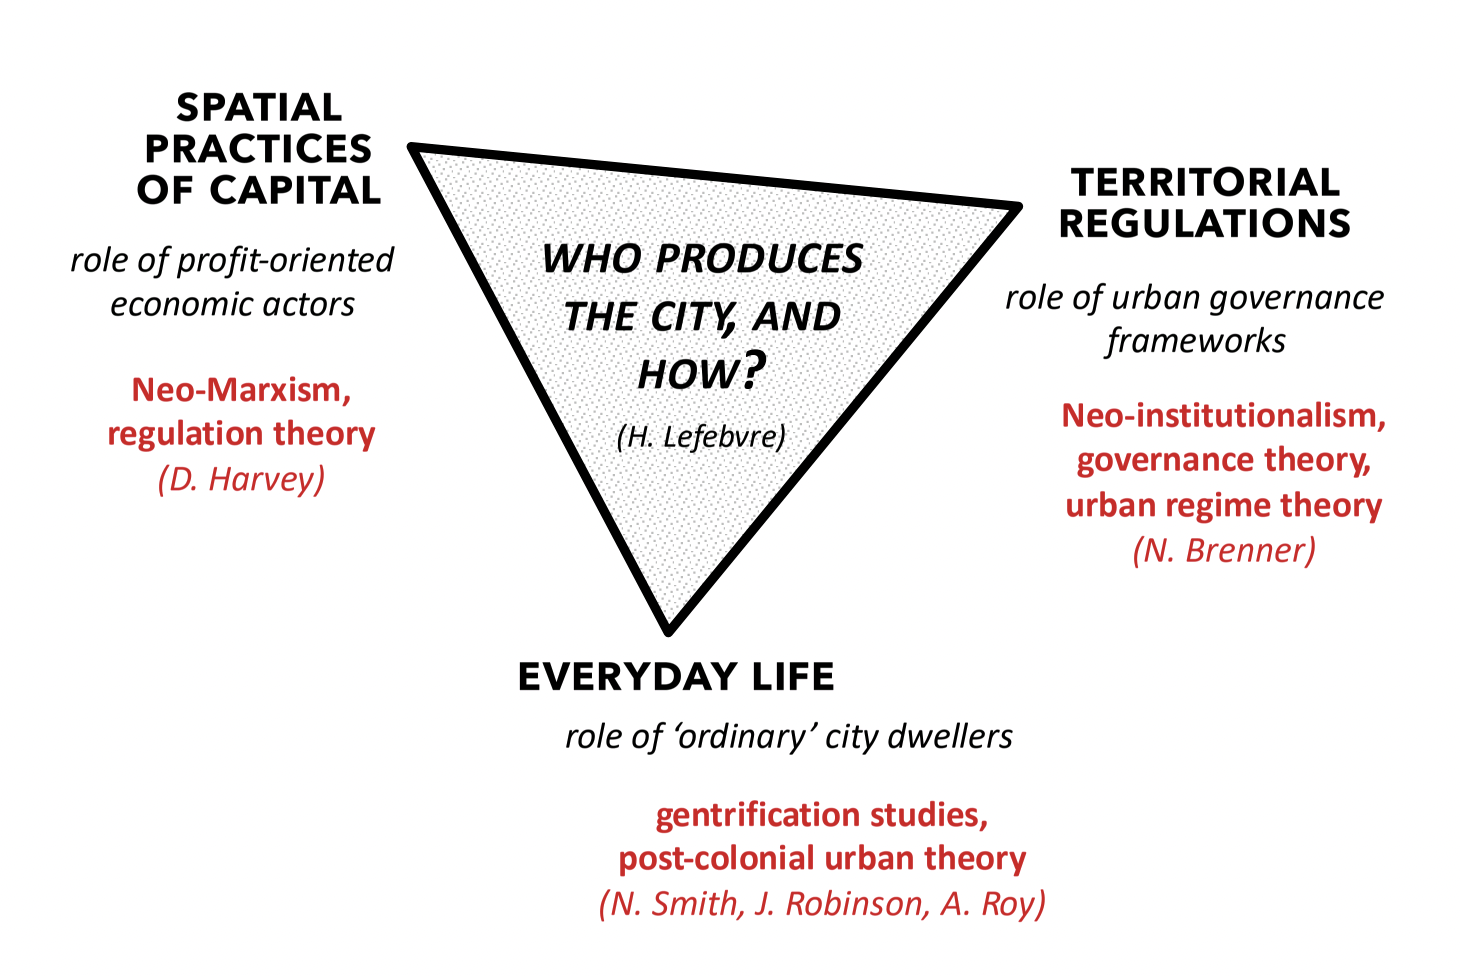
\includegraphics[width=\textwidth]{map_course_organisation1}
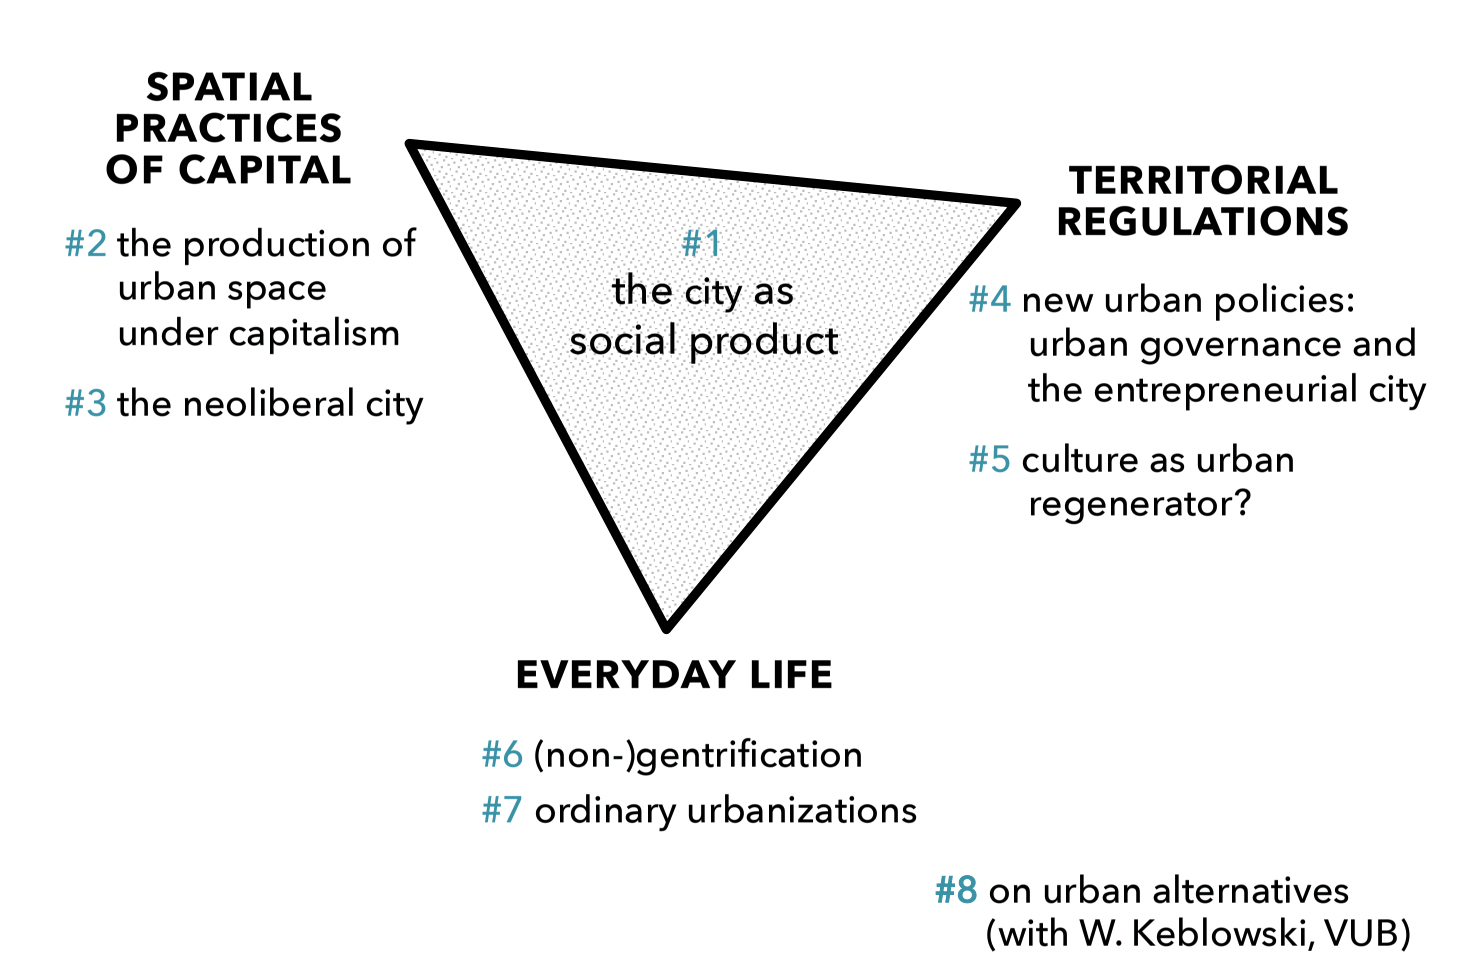
\includegraphics[width=\textwidth]{map_course_organisation2}

%%%%%%%%%%%%%%%%%%%%%%%%%%%%%%%%%%%%%%%%%%%%%%%%%%%%%%%%%%%
% 																			 LECTURE 2
%%%%%%%%%%%%%%%%%%%%%%%%%%%%%%%%%%%%%%%%%%%%%%%%%%%%%%%%%%%

\section{Spatial Practices of Capital}

\section{The Production of Urban Space Under Capitalism}
\date{October 7th, 2021}

\textit{tldr; Harvey's theory of the production of urban space under capitalism}

\subsection{Evolution of Urban Space}

What do you think about when you think of urban landscapes? $\rightarrow$ standardisation and copy/past urbanism, shopping streets, high streets; gated communities, suburbanisation, landscapes of dispossession; Dubai, skyscrapers, American malls with extensive parking lots; inequality landscapes; CBD (Central Business District)

We could think of:

\begin{outline}
	\1 Shanghai: from 1990 to 2014, it became a metropolis, China entered the world trade organisation and became a super power
	\1 Panama City: from 1930s to 2010s, became a haven for tax-evasion and offshoring of wealth; came to light with Panama papers
	\1 Cleveland Ohio: in 2008, had many foreclosures due to financial crisis, landscape of abandonment and dispossession 
\end{outline}

\subsubsection{David Harvey}

David Harvey had a theoretical project \textbf{``to integrate an understanding of processes of urbanisation and built environment formation into the general theory of the laws of motion of capital''}, ie. how does urbanisation help us understand capitalism.

He asks the questions:

\begin{outline}
	\1 How and why does capitalism (re)shape (urban) space?
	\1 What's structural about the urbanisation of capitalism, and what's historically/geographically contingent?
	\1 How does the restless character of capitalism (crises, booms, busts...) affect cities?
	\1 How and why does the capitalist production of space bring uneven spatial development?
\end{outline}

\subsection{Capitalism and urbanisation}

\subsubsection{Capitalism}

Capitalism is a system of economic production based on the circulation, or exchange, of privately-owned capital and geared towards capital accumulation. 

Under capitalism, you must re-invest your profit, otherwise other actors will out-compete you (and put you out of business). You also want public or private investors to invest in your business, and such financial investments have grown so much as to become problematic\footnote{The financial investment space is not something I understand well; general understanding is that banks, or finance institutions, lend money/invest, ie. give credit, which means the businesses/people must pay back this money plus interest, and this means they must make a profit. And this has become a problem, because loans cannot be paid back correctly or on time?} 

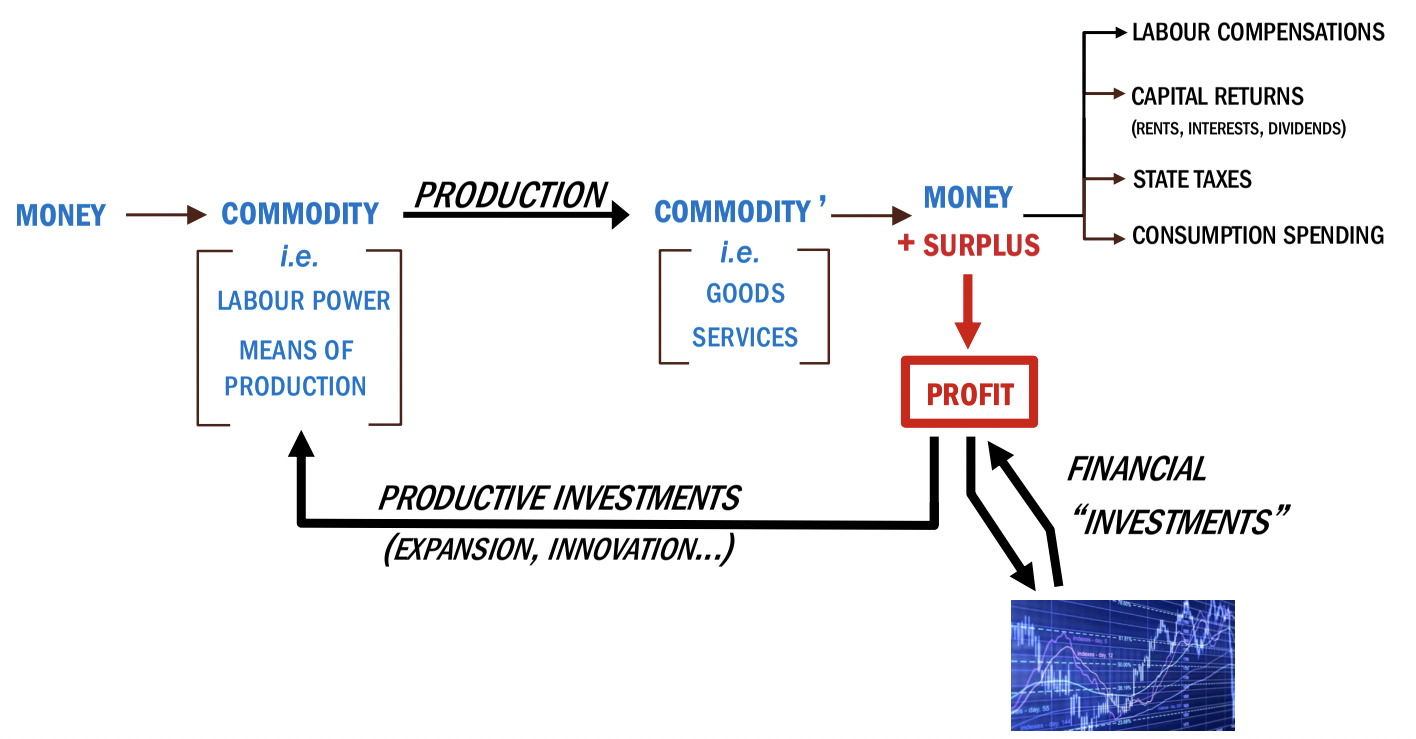
\includegraphics[width=\textwidth]{capitalism}

Thus, capitalism:
\begin{outline}
	\1 An ever-expanding system: capitalism must grow
	\1 Has a geography: it isn't the same everywhere, it's embedded in varying social, cultural, institutional configurations (eg. colonial capitalism, war capitalism, State-controlled capitalism...)
	\1 Has a history: it evolved over time, from a merchant capitalism (16-17th century) $\rightarrow$ liberal industrial capitalism (18-19th century) $\rightarrow$ Fordist/Keynesian industrial capitalism (20th century) $\rightarrow$ neoliberal capitalism (late 20th century)
\end{outline}

%\subsubsection{Capitalism and urbanisation} 

Can we say that cities are created by capitalism? No, cities are not creations of capitalism and existed prior to it. However, the rise and extension of capitalism is deeply linked to the urbanisation process: the emergence of merchant capitalism in Europe's medieval cities, and the massive urban transition since the rise of industrial capitalism, are two eras where capitalism sped up urbanisation.

\subsubsection{A crisis-prone system}

Capitalism is crisis prone, but it has been resilient through history\footnote{China's Evergrande crisis: the collapse of China's second biggest property developer created fear that China's financial system could collapse, however, it did not.}. 

\begin{outline}
	\1 Accumulation is at risk when surplus capital has no outlet in sight for profitable reinvestment, because the circulation of capital cannot continue
	\1 If an outlet is not found, the financial bubble crashes, there are plant closures, social upheavals, geopolitical conflicts...
\end{outline}


Harvey focuses on capitalism's crises. His guiding question is, throughout history, how has capitalism emerged from its periodic crises and found ways to expand further?

\subsection{A theory of urbanisation under capitalism - `fix'}

A `fix' can be one of three things: to put something in place; to repair something; to satisfy an addiction. In capitalism, a fix is a \textbf{temporary `solution' to capitalism's inner crisis tendencies.}

\textbf{Technology fix}: reinvestment of surplus of capital in new or improved production capacities, ie. new sectors and products fuelled by technological and organisational innovations $\rightarrow$ new rounds of growth

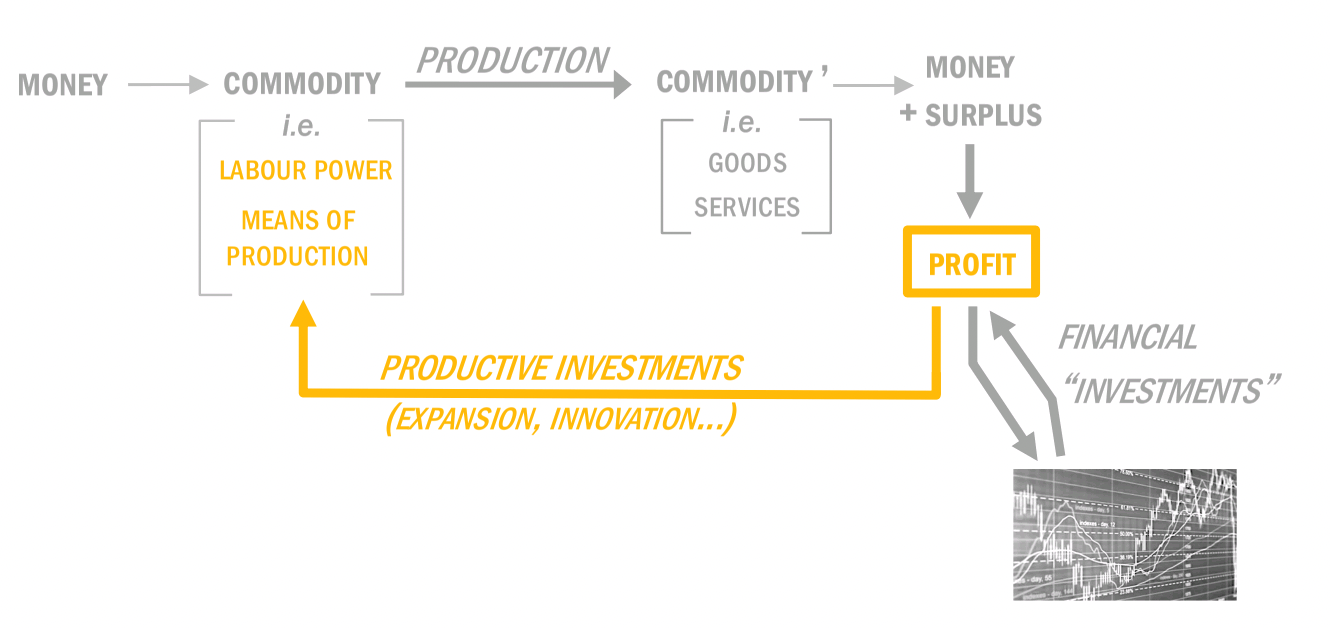
\includegraphics[width=\textwidth]{technological_fix}

\textbf{Financial fix}: reinvestment of surplus capital into financial assets (shares, securities, debt claims...) for the sake of rents and capital gains. This is `financialisation' of capitalism\footnote{For financialisation of capitalism, refer to class no. 3}

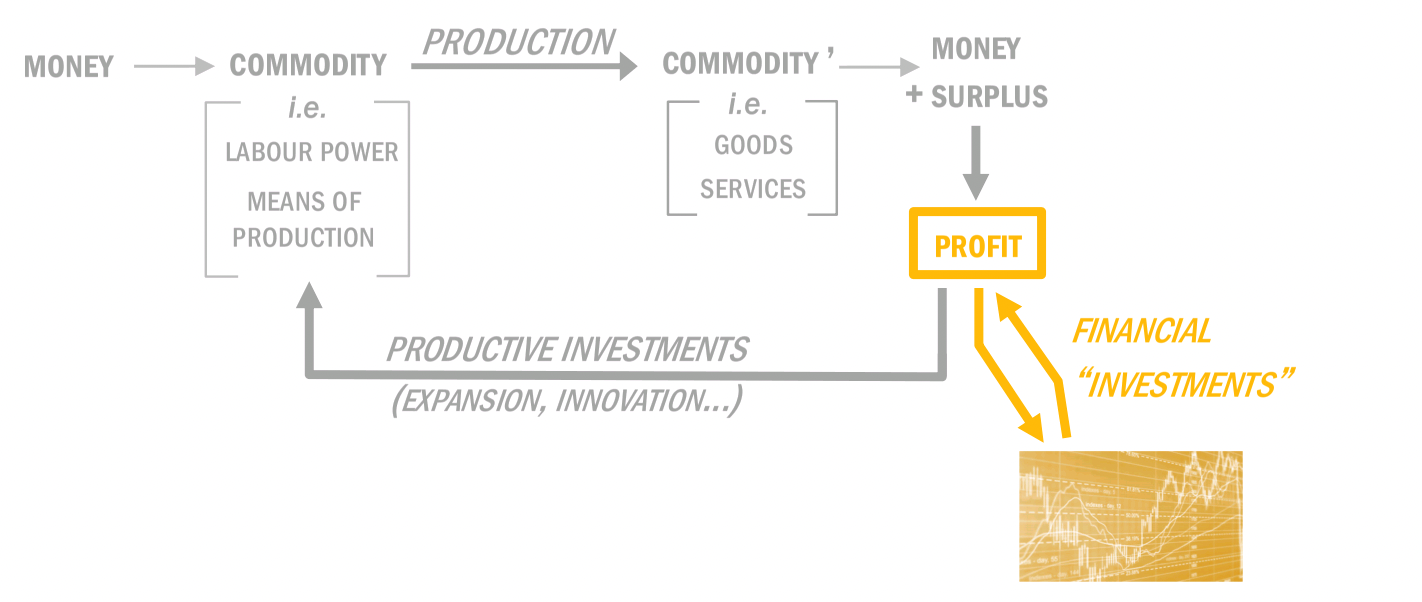
\includegraphics[width=\textwidth]{financial_fix}

\textbf{Spatial fix}: injecting surplus capital into the production of profitable investments. We can observe that the peaks of the construction of tall buildings are not randomly distributed, and are higher at times of crisis (1930s, early 70s, late 80s-90s during the dot com crash and its over optimism, 2008 subprime mortgage crisis).

China and the UAE have the highest number of skyscrapers, and at the same time are places where massive capital surplus exists (or existed at time of building).

\subsubsection{A theory of urbanisation under capitalism}

\begin{enumerate}
	\item Volumes of capital are invested in a selection of localised built environments, in sync with macro-economic temporalities
	\item There is a paradox: investment volumes in the built environment peak in crisis time
\end{enumerate}

Harvey's point is that under capitalism, urbanisation is essential to over capitalism's inner contradictions. \textbf{The production of space is a key outlet for surplus capital and profitable reinvestment} (= spatial fix). ``Capitalism ... is addicted to geographical expansion much as it is addicted to technological change and endless expansion through economic growth''.

The addiction the geographical expansion is both horizontal (taking up more surface area), and vertical (buildings are as high as possible to take in the highest number of people or businesses).

Capitalism is after new spaces of industrial production, of transport and logistics, of consumption, of rent speculation, and new urban markets (eg. airbnb\footnote{In Brussels, Airbnb represents $<$1\% of the housing market, relatively small but Brussels isn't the biggest tourist destination; it is unequally distributed throughout the city, and is concentrated in the city centre, the EU quarter, and the train stations; Airbnb created a new market, which was originally a sharing economy (sharing a room when you are away)}).

\textit{Will this theory still apply when almost all of the world is urbanised?} Yes, because there is creative destruction of urban space. NYC was completely urbanised int he 80s, yet continues to grow through creative destruction. 

\textit{What is a profitable development?} A development that absorbs capital surplus and surplus labour force. It will bring capital back to the investors, who invest speculatively. For the sake of `fixing' capitalism, the fix is consumed as soon as the capital is spent in the development, even before the development is completed and profit has come. 

\subsubsection{Any fix is short-lived}

Under capitalism, any fix is short-lived, temporary. 

\begin{outline}
	\1 Paris' Haussmannisation, 1853-1868: Paris was in a time of severe crisis, with the revolution in 1838. Napoleon III arrives rises to power in 1852 and appoints Haussmann to develop the city. 
		\2 Haussmann develops profitable outlets like the Grands Magasins, the Opera
		\2 There is a massive transformation from the medieval character of Paris (tiny, dirty streets) to grand, clean avenues
		\2 This type of development requires a massive amount of capital
		\2 In \textit{The Housing Question}, 1872, Engels questions the legitimacy of Haussmann: the plan was to make Paris more liveable, but did it consider the people who were currently living there? Will they be back in the new buildings that replaced the `slums' and `ghettos'?
	\1 Post-war capitalism and urbanisation (jobless demonstration in Chicago, in 1934)
		\2 Technology fix: investment in mass production of durable consumer goods by industries organised along Fordist principles, to be consumed by expanding national customer markets supported by Keynesian economics
		\2 Financial fix: massive allocation of capital into the credit system, towards companies, households (mortgage credits, consumption credits) and State authorities (debt-financed public works and infrastructure, eg. New Deal, Marshall Plan)
		\2 Spatial fix: massive investment in urban expansion (housing, infrastructure, highways) fuelling a huge wave of suburban growth centred on middle-class habitat and consumption patterns
\end{outline}

\subsection{Suburbanisation}

Picture LA, with miles and miles of single family housing; the American dream of owning a private house with a backyard and a car, almost regardless of the commute and community (or lack thereof);

See \textit{Suburban Planet}, Roger Keil.

Suburbanisation is not a middle-class phenomenon. Low income households are now moving away from dense urban centres, especially when inner-city neighbourhoods become gentrified and expensive.

\subsubsection{The case of Belgium}

Belgium's policies favoured the development of housing along the motorways that connect cities together, and it is a particularity of Belgium to have a lot of motorways (0,2km of motorway per person in Belgium, twice as much as in France). The intense development of the motorways created a favourable environment for Belgians to built their own house, and the ideal became to have a house `far away' from another, with a (company) car (preferably a company car). 

There is a saying that ``Belgians have a brick in their stomach'', meaning that they are born wanting to build a house.

\subsection{Summary the theory of urbanisation under capitalism}

\begin{outline}
	\1 Capitalism has an \textbf{insatiable addiction to the production} of (profitable) space, for this is a key way to overcome its own contradictions
	\1Under capitalism, \textbf{the mobilisation of urban change for the sake of capital accumulation is permanent}, but lays at the forefront in crisis times
	\1 Under capitalism, \textbf{any spatial fix is short-lived}, for the (profitable) way out of a crisis paves the way to the next crisis
	\1 Under capitalism, \textbf{fixing space has ramifications}, on the built environment but also on modes on consumption, mobility patterns, cultural and political subjectivities
	\1 \textbf{Under capitalism, any spatial fix comes with patterns of uneven spatial development}
\end{outline}

\subsection{Uneven spatial development}

Under capitalism, patterns of investment in some places are structurally associated with patterns of \textbf{disinvestment} elsewhere. Creative destruction displaces communities who are not allowed to return afterwards.

\begin{outline} 
	\1 t0: selected places are dynamic edges of capitalist urbanisation, for their production participates in a spatial fix
	\1 t0 $\rightarrow$ t1: progressively, those places lose their fit vis-a-vis evolving capital requirements
	\1 t1: capital fixed in the those places is devaluated, for new places are now more profitable for investment, or they become local barriers to new rounds of accumulation
	\1 t1 $\rightarrow$ t2: capital moves elsewhere, or is invested in a `creative destruction' of local space
	\1 t2: capital moves back in restructured places, that appear attractive once again under new circumstances
\end{outline}

There is a cyclic dimension to the spatial fix: capitalism doesn't solve crisis, but moves them around geographically. 

Take the examples of Ny-Lon-Kong (NY, London, Hong Kong) and Detroit. These two places are part of the same story. The investment in one causes the disinvestment in another.

\url{https://www.youtube.com/watch?v=qOP2V_np2c0&ab_channel=RSA}

\subsection{Keywords}

David Harvey
Capitalism
Capitalism's crisis
Production of space
Fix: technological, financial, spatial
Keynesian economics
Creative destruction

%%%%%%%%%%%%%%%%%%%%%%%%%%%%%%%%%%%%%%%%%%%%%%%%%%%%%%%%%%%
% 																		 LECTURE 3
%%%%%%%%%%%%%%%%%%%%%%%%%%%%%%%%%%%%%%%%%%%%%%%%%%%%%%%%%%%

\section{The Neoliberal City}

\textit{tdlr; zooming in to the present conjuncture of the production of space under capitalism, ie. urbanisation under neoliberal capitalism, or the `neoliberal' city. Urban spaces are sites and vehicles for neoliberalism: sites because that is where the accumulation takes places, and vehicles because of the financialisation of the real estate market, and it's speculation. The 21st century city is a city of rents.}

\textbf{Why is housing so expensive in cities?} 

\begin{outline}
	\1 There is a problem of \textbf{supply and demand}: prices are pushed up when the demand is high and the supply low (economic argument). The logical solution would be to boost supply, but interest rates are too low and so people are not selling their properties.
	\1 According to neoliberalists, there is \textbf{too much regulation}, and investors cannot supply enough properties. Exclusionary zoning prevents multi-family housing, there are height restrictions, parking requirements drive prices of housing upwards (for 100 housing units, you need 200 parking spots, which is not possible to find space for anyway). 
	\1 Conservative residents, \textbf{NIMBYs}, participate in community meetings regarding housing developments, and protest against changes
\end{outline}

But, focusing only on supply and demand is limiting. For example in Berlin, the demand is low but the prices are rising. In London, the prices are rising but real estate is also increasing.\footnote{What happens in places where space is not an issue, for example, in Astana?}\marginpar{Astana has `unlimited' space - how does that affect housing market?} 
Renting is a \textbf{``second hand market''}.

\href{https://www.vox.com/22629826/gentrification-definition-housing-racism-segregation-cities}{Vox:  What we talk about when we talk about gentrification}

\subsection{What is neoliberalism?}

Neoliberalism is ``the set of intellectual proposals and political orientations that aim to extend market mechanisms and ethics of competition to an every-wider spectrum of social activities, based on strong state intervention'' (Pinson, 2020)\marginpar{Neoliberalism is the extending of markets, based on state intervention}

Neoliberalism isn't about the privatisation of everything, it isn't `laissez-faire'. 

\begin{outline}
	\1 Neomarxism: neoliberalism is a \textbf{class project to remove restrictions in the way of accumulation} (Harvey)
	\1 Bourdieusian: a State project, with state interventions (Wacquant)
	\1 Foucaldian: a new ethos, or government rationality (Brown)
\end{outline}

\subsection{What's new about neoliberal capitalism}

\subsubsection{20th century trend of capital in the Global North}

From the 1980s, there is a turn from the Fordist-Keynesian era to the \textbf{`post-Fordist', `informational', `flexible', `globalised',... `neoliberal' era}. 

Pre 1980s, the profit rate decreased, and there was a capitalism crisis. Then, things took a \textbf{neoliberal turn}:

From the early 1980s, the profit increased, but the reinvestment rate was low. There is still a growing gap between the \textbf{profit rate} (the return on productive capacities) and the \textbf{accumulation rate} (the share of profit reinvested in productive capacities). Capital has grown, but has not been accumulated (reinvested).

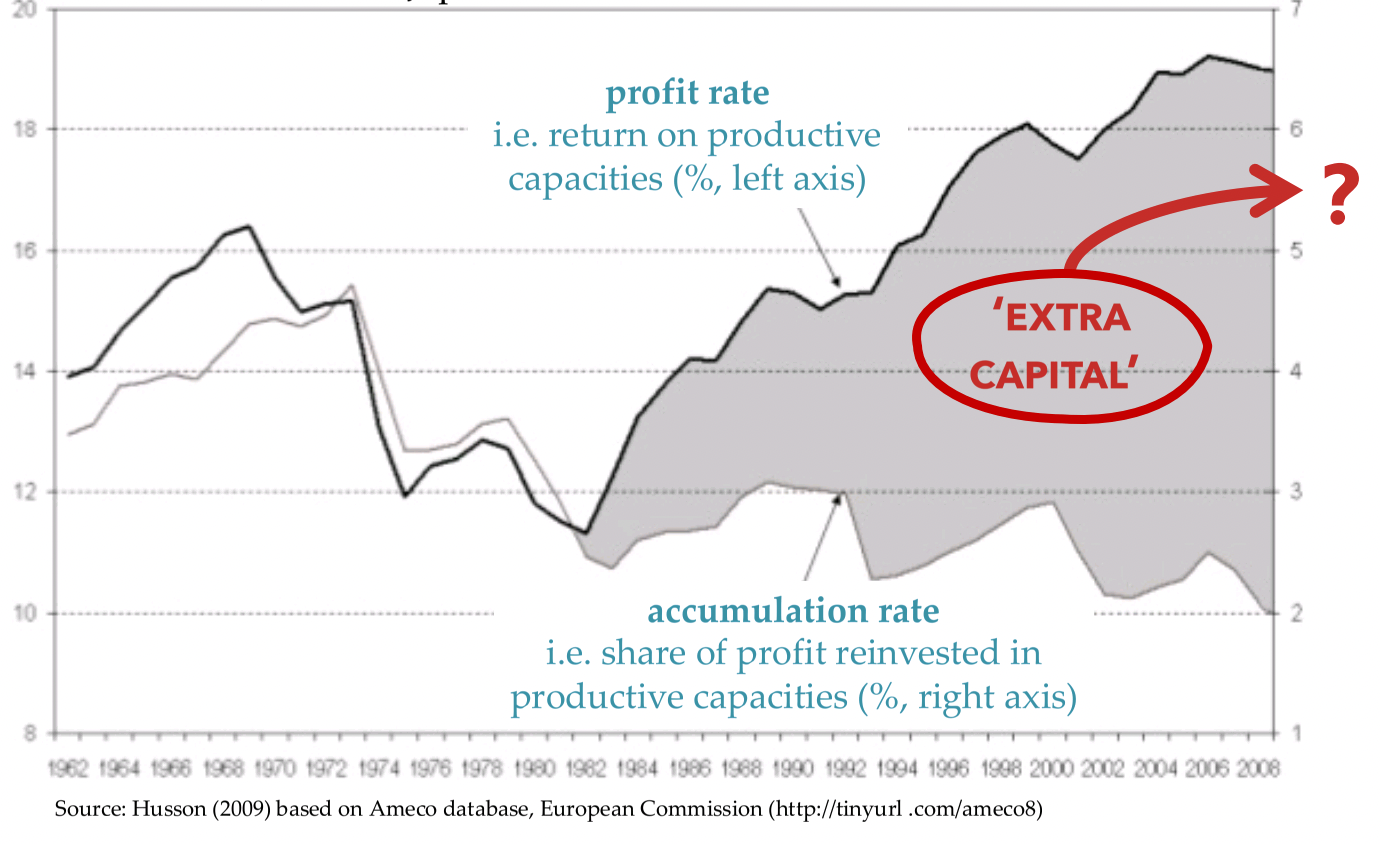
\includegraphics[width=\textwidth]{neoliberal_turn}

The question is, \textbf{what happened to this surplus of capital?} 
It was not reinvested in wages, and taxes did not increase. 

\subsubsection{The surplus of capital}

There was a \textbf{trans-nationalisation}, where capital was invested externally: companies globalised, off-shored and outsourced their production, there were mergers and acquisitions, foreign direct investment

There was also a switch to \textbf{financialisation} of capital, where the surplus went into financial markets

\subsubsection{Transnationalisation}

An increase in Foreign Direct Investment (FDI), ie.  investors establishing long lasting interests in an enterprise residing in another country. 

\subsubsection{Financialisation}

The Dow Jones is a collection of traded companies, ie. companies available through the financial market. Since the 1980s, its value has grown enormously, showing how enormous financialisation has become.

Financialisation:

\begin{outline}
	\1 Is an increasing concentration of capital in the financier's hands
	\1 Uses \textbf{asset valuation} strategies, where the purpose is to valorise a set of assets (what ever an asset can be) and speculate, and thus maximise rental\footnote{Rent is the payment charged by the owner of a property, to a user, in return for its use} yields (dividends, rental income, interest returns...) or capital gains on resale
\end{outline}

Comparing GDP of countries with the largest asset managers, if Germany was an asset manager, that is if all of the German companies (Mercedes, Audi, BMW, etc.) formed an asset management company, they would the 3rd biggest in the world. This shows how huge the concentration of wealth is in financial circles. 

\subsection{In what sense is neoliberalism urban?}

Cities and urban spaces are \textbf{strategic and critical} for neoliberalism:

\begin{outline}
	\1 as critical \textbf{sites} of capital accumulation
	\1 as critical \textbf{vehicles} for capital accumulation
\end{outline}

\subsubsection{Critical sites of accumulation}

\begin{outline}
	\1 \textbf{Global cities}\marginpar{S. Sassen} need to control ever more of the world networks and flows
		\2 There is a \textbf{spatial concentration of strategic command and control functions}
		\2 They are nodes in a global space of flows (money, information, goods, services, workers...). Being an entity in one global city, brings you closer to peers in other global cities, rather than bringing you closer to peers who are geographically closer, but who's city is not global $\rightarrow$ a network of people between global cities, that excludes others from participating if they do not have the same `power'
		\2 Global cities are biased to the Global North
	\1 \textbf{Worlding cities} (A. Roy, A. Ong) are cities emerging as global cities
		\2 Typically from the Global South, and from emerging countries (Shanghai, Singapore, Hong Kong, Taipei, Mumbai, Doha, Dubai, Rio de Janeiro, Johannesburg...)
	\1 \textbf{Globalisation from below} (A. Portès) 
		\2 Places of production and consumption associated with transnational communities sitting astride political borders
		\2 For example, Marseille, or Rue Heyvaert in Brussels where European cars are shipped to North Africa and the Middle East
	\1 \textbf{Inconspicuous cities beyond global cities} (A. Choplin, O. Pliez)
		\2 Secondary cities should be given more consideration
		\2 Global cities invest in such cities, and thus they are crucial for how capital accumulation works
	\1 \textbf{Urban peripheries}
		\2 Global suburbanism (R. Keil)
		\2 Planetary urbanisation (Brenner and Schmidt) is about the implosions and explosions, the concentration and the extension of urbanism. Planetary urbanisation means that spaces that are far away from the city cores and suburban peripheries, are strongly linked to urbanism and urbanisation. For example, Alberta, Canada's oil fields are fuelling an urban lifestyle
\end{outline}

\subsubsection{Critical vehicles of accumulation}

The Battersea Power Station in London sold for 1.6bn gbp to a Malaysian fund. The power state is a landscape of cranes, building housing units/leisure/business spaces, but it isn't a local project.

\begin{outline}
	\1 There is a growing \textbf{financialisation} of urban development
		\2 Huge amount of capital goes into commercial real estate markets (retail, office, housing, logistics) since the late 1990s
			\3 Capital switched around the 2000 dot com crash, from internet companies to real estate (leading to the subprime mortgage loans)
			\3 This led to the subprime mortgage crisis, and we see that one crisis creates another
			\3 Highly uneven geography, where Global North and global cities have significant investments, and \textbf{capital converges} 
		\2 Increased coupling of real estate activity to market finance
			\3 Rise of real estate asset management
			\3 Strategies of \textbf{assetisation}, to turn real estate (land, property) into financial assets to be treated as such
	\1 From assetisation of real estate to \textbf{speculative urbanisation}
		\2 The mobilisation of land or property for the sake of maximising rent extraction.
		\2 Speculation is trying to extract as much money from your property. Land is mobalised
		\2 The 21st century metropolis is a \textbf{city of rent}\marginpar{Samual Stein, \textit{Capital City}}
\end{outline}

\subsection{The 21st century city of rent}

There are multiple expressions:

\begin{outline}
	\1 The rise of corporate landlords and buy-to-let housing markets
	\1 Speculative projects tailored to meet investor's requirements first
	\1 Increased tendency of urban governments to rely on the real estate valorisation of their land resources in order to finance public utilities
	\1 Growing un-affordability as a systemic feature, because profit is necessary
		\2 Highlights the uneven geography, as investments rise in one place (= city growth) and leaves other places behind (= shrinking cities).
\end{outline}

\textit{\textbf{$\Rightarrow$ Neoliberal urbanisation as “neo-Haussmannization” (Merrifield, 2014), “generalized gentrification” (Smith, 2002), “planetary gentrification” (Lees, Shin, Lopez-Morales, 2016), a regime of “expulsions” (Sassen, 2014), “accumulation by dispossession” (Harvey, 2003)}}

%%%%%%%%%%%%%%%%%%%%%%%%%%%%%%%%%%%%%%%%%%%%%%%%%%%%%%%%%%%
% 				 LECTURE 4
%%%%%%%%%%%%%%%%%%%%%%%%%%%%%%%%%%%%%%%%%%%%%%%%%%%%%%%%%%%

\section{Territorial Regulations}

\section{New Urban Policies: Urban Governance and the Entrepreneurial City}

\textit{tldr; capitalism isn't the only force shaping the city. Urban governance and the entrepreneurial city play an increasing role in shaping urban space}

\subsection{Making sense of the role of the State in contemporary urban changes}

To think capital alone shapes cities is too simplistic, because it's not only an economic structure that shapes the urban.
There are multiple ways to make sense of the role of the State in contemporary urban change:

\begin{outline}
	\1 \textbf{Neo-institutionalism}
	\1 The \textbf{neoliberalisation of urbanism} (compared to the urbanisation of neoliberalism,  lecture 3)
	\1 \textbf{Creative destruction of the State} (compared to the creative destruction of economic structures, lecture 3)
\end{outline}

We need to consider a much broader range of public actors, and those interacting with state institutions (NGOs, lobbies, etc.).

So, what's new with recent urban politics? 1. The rescaling of statehood, 2. The rise of urban governance, 3. The rise of urban entrepreneurialism.

\subsection{Rescaling of statehood}

Brenner\footnote{Neil Brenner, \textit{New State Spaces}} follows Harvey's theory, and puts more emphasis on \textit{the role of the State} in the production of space in the capitalist regime.

His core argument is, that the re-configuration of economic structures (1980s) went hand in hand with the \textbf{re-organisation of the scales of State regulation} of capitalism, ie. a \textbf{rescaling of Statehood}. Statehood is the whole set of logics of actions and mechanisms through which public power is exercised. 

The difference between the State and statehood, is that State is an institution, and statehood is an abstract idea. Statehood represents public power, public authorities, and all the forms through which public power is exercised. It is detached from a specific scale.

There is the emergence of less national-centric form of statehood in capitalist countries. National states have not been eliminated, but this rescaling in public regulation (eg. of capital flows), has brought more importance to other scales than national one:

\begin{outline}
	\1 \textbf{Upscaling}: towards supra national tiers of government (eg. EU)
	\1 \textbf{Downscaling}: devolution, towards sub-national tiers (eg. Belgium regions, Dutch provinces, German Lander, agglomerations)
	\1 \textbf{Outsourcing}: towards private and civiil society actors
\end{outline}

All together, the complete picture is an increased relevance of urban/regional scale of State power (statehood), regarding the production and development of urban policy.
The global architecture of State power is multi-layered, and the urban scale has a greater importance than before.

This rescaling is visible through the new transnational network of city governments\footnote{Eg. Euro Cities, Euro Cities' Mayor Summit, C40 cities (climate leadership group), Resilient Cities Network, Global Parliament of Mayors)}. Usually, such transnational organisations exist on the nation scale, and not the city.

Brenner's point of the rescaling of statehood is not like the ``triumph'' or ``revenge'' of the city (Glaeser), where governments need (and aren't able) to face the challenges of 21st century.
Rather, it is about the \textbf{emergence of a multi-layered, less national centric form of Statehood} within which the urban/regional scale plays more important and autonomous political/economic role than previous decades.

In the background, there is a retraction of (less) national-to-local transfers of investment capacities.\footnote{For example, the vision of North Quarter in Brussels in the 1960s. The North Quarter was supposed to be transformed into a global financial centre, mimicking NYC's  world trade centre. However, the development of world trade towers in Brussels was s complete failure, and the consequences are still visible: the Northern Quarter is not a great, liveable place. At that time, such developments were made at the national level. This would not happen anymore, since the scale of ``who decides'' is completely different, and the role of regional authorities is central now. Ie. there is a \textbf{rise of urban governance}}

\subsection{Rise of urban governance}

The use of `governance' instead of `government' is to represent a diversification and widening of stakeholders involved in urban policy making.

Urban governance reoriented the debate on political power in cities, beyond Government and Parliament, towards a production of the \textbf{``capacity to govern''}\footnote{C. Stone, \textit{Regime Politics}, 1989}. People who have the material and symbolic capacity to govern, may not be the ones in the seats of government.

\subsubsection{Urban regime theory}

Urban regime theory assumes that no one in the city holds all the resources and capital necessary to have enough impact to produce urban policy, and urban projects. The \textbf{capacity to produce is distributed} amongst a wide range of actors of various types, operating at multiple scales, and controlling/bringing to the table specific resources (legislative, politic, economic, symbolic...).

\textbf{Urban politics} is the activity of assembling these resources (stakeholders, institutions,...) together, and find a consensus, ie. to compose an effective capacity to govern with a certain stability (eg. for a certain amount of time). An urban regime is a set of (in)formal  arrangements, that enable multi-stakeholder coalitions. There is no `office' of the urban regime, rather, a network of people across space.
The stakeholders all have the common interest of growing the economy.

\textbf{Tour et Taxis}

Tour et Taxis was an industrial site, for warehousing, freights, with large rail station for goods but not people. It was emptied in the 1980s, and has been under redevelopment since then.

It's a historic site that was supposed to be a multifunctional neighbourhood with housing, offices, leisure, event spaces, green space... the largest development in Brussels.

Who is developing this? A shareholding company bought it from the port authority; the company gets money from bank institutions and investors, and using this money, they bring in construction companies; they have important tenants (eg. administrations), events are taking place (attracts people, the media, radio stations), the site is in the Brussels region, but regional government is also involved,... and the involvements go on. Tour et Taxis is a \textbf{multi-stakeholder project}.

Through what channels does this ``assemblage'' become effective? There are multiple channels for assembling urban governance frameworks:

\begin{outline}
	\1 \textbf{Public-private partnerships}: PPP, eg. Villo which is a partnership between Brussels region and JCDecaux
	\1 \textbf{Citizens' participation frameworks}
	\1 \textbf{Strategic planning}
\end{outline}

\subsubsection{Public-Private Partnerships, PPP}

A PPP is a legally binding, contractual arrangement between an \textit{ad-hoc} private actor (contractor) and a public authority, for the development of an equipment of public interest, over a fixed period of time (eg. 25 years).\footnote{Eg. Øresund bridge between Malmö and Copenhaguen}
 
Most often, the private contractors have DBFM-O contracts. This means they design, build, finance, maintain and operate the project, via a dedicated project-based operating structure, against the payment of a yearly feel by the public authority due for a fixed period (eg. 25 years).\marginpar{Are Astana buildings PPP?}

At the end of the contract period, the public authority becomes the full owner of the (eg. 25 year old) equipment.

The public authority also contributes with land allocations, tax cuts... And the users often pay a fee for the facility, to compensate for the fee that the contractors pay.

Pro arguments:
\begin{outline} 
	\1 It limits public indebtedness, because the public authority doesn't have to borrow money in the first place. It's a way around the limitations on public borrowing, in the name of `healthy' public finances and not passing debts to future generations
	\1 The public authority doesn't have to fund the civil servants to run the facility, because the PPP will take care of it. Using the existing private management structure, instead of public administration, reduces operating costs and is assumed to be more effective
\end{outline}

Contra arguments:
\begin{outline}
	\1 More costly for public finance in the long term, compared to a classic bank loan; you have to pay the contractor, plus their profit (a fee) because private contractor seeks a return on investment
	\1 Not hiring civil servants is a loss of expertise on the part of the public administration, regarding development and operational management of infrastructure and equipments
	\1 Empowers private actors to direct and influence the allocation of public funds
	\1 Harder times for parliamentary control of the government's spending, which raises issues about democratic control. PPP contracts are confidential and not public documents, and operators are not accountable to the Parliament
\end{outline}

Some governments have decided to not use PPPs for infrastructures such as hospitals. After 30 years of private ownership, when the ownership of the site is transferred to the government, there is no guarantee of the state of the equipment.

\begin{center}
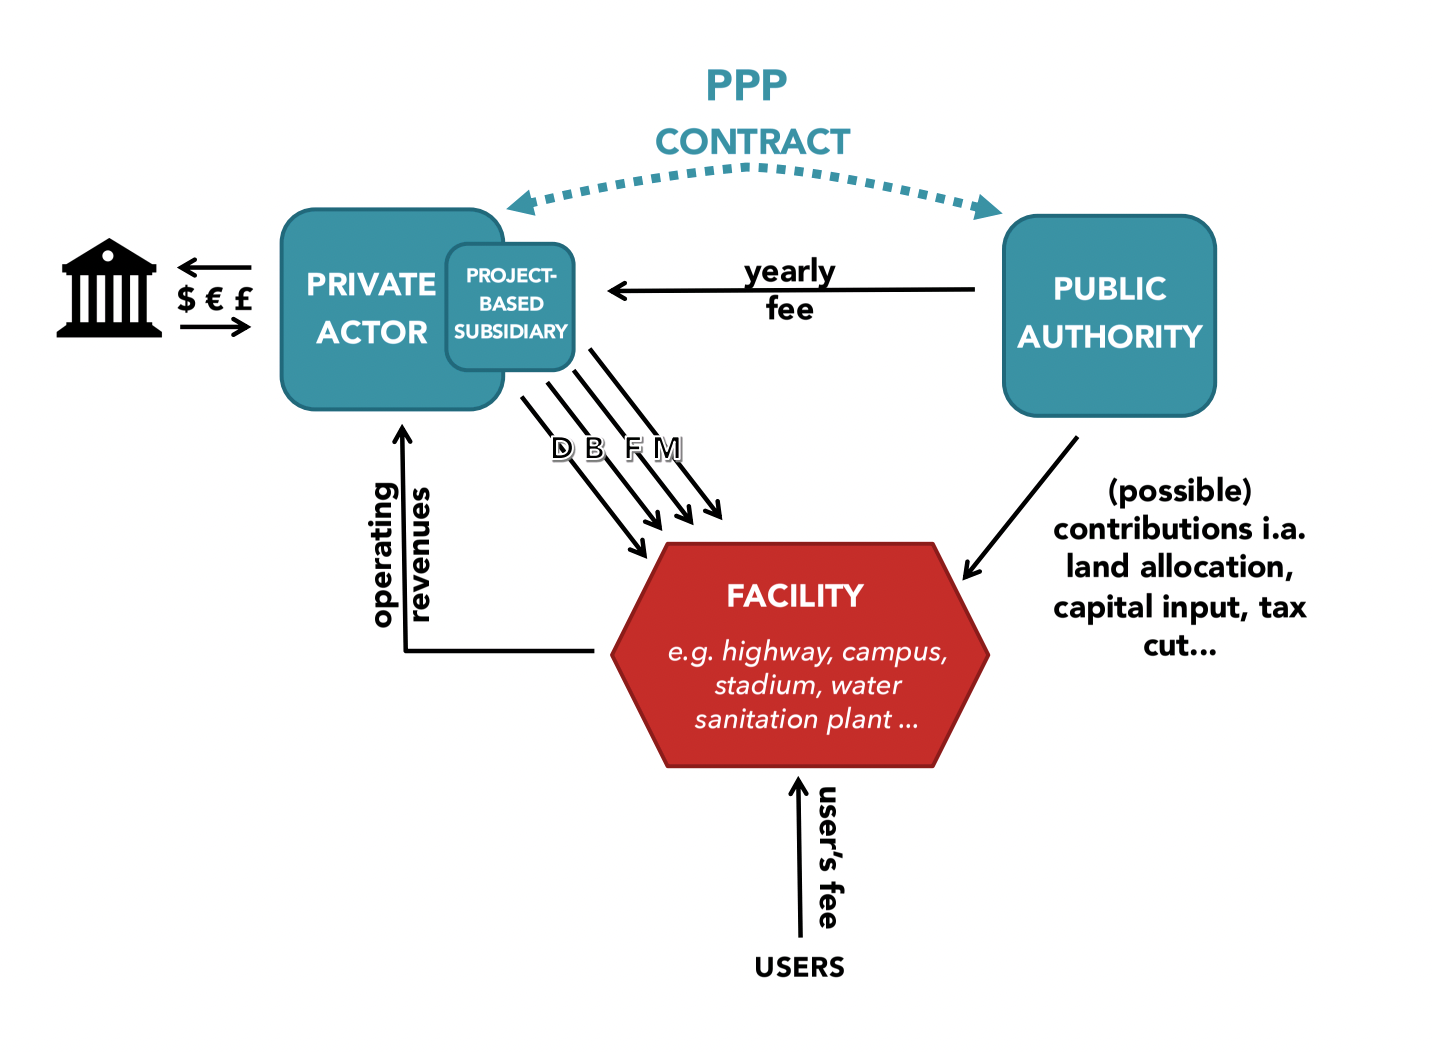
\includegraphics[width=35em]{public_private_partnerships}
\end{center}

\subsubsection{Citizen participation framework}

\textbf{``Participatory turn''} in urban politics are platforms, councils, assemblies, forums, debates, hearings, consultations, workshops, walks...

The rationale is to bring policy-making closer to the people, to be more `open' and `responsive' to citizens. This can bring fresh ideas, and ease project acceptance and reduce opposition through information and dialogue.

Recurrent limitations and biases:
\begin{outline}
	\1 Some categories of populations participate more than others, and are given more rom. There are class, gender, ethnic, demographic, owner/renter, etc. biases
	\1 Equalising levels of information between participants (experts vs. inhabitants) requires more time and energy than is usually spent. There are time tensions, because the political and electoral agendas have short terms, and running the participatory turns properly would take too long. Instead, politicians want them to be a fast process, but the experts' speed is much too quick for the participating inhabitants
	\1 `Local trap': debates are often directed towards local solutions (neighbourhood scale) which keeps the wider picture out of sight and discussions. This is a problem because not all local problems can be solved locally, and sometimes involved processes that are supra-local
\end{outline}

S. Arnstein's \textit{A Ladder of Citizen Participation} asks, how much power is actually transferred to citizens in the participatory frameworks?

\begin{center}
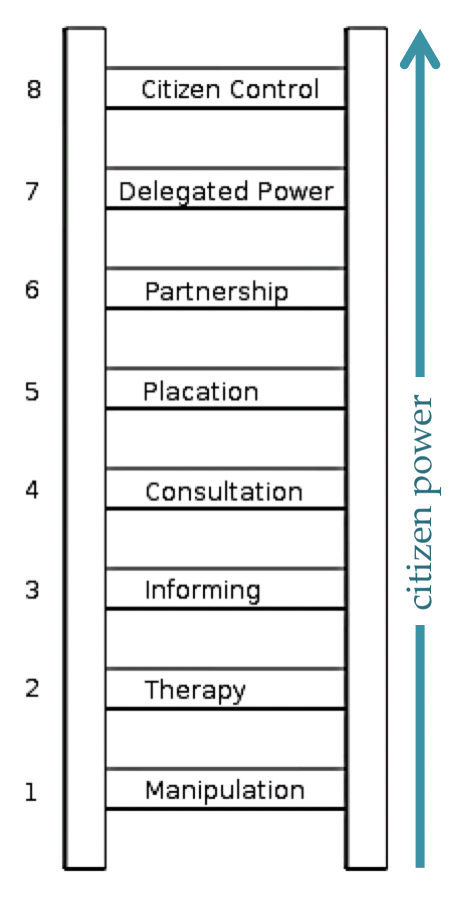
\includegraphics[width=10em]{citizen_participation}
\end{center}

\subsubsection{Strategic Urban Planning}

A `strategic' or `project based' turn in urban planning.

A \textbf{land use map} is a map where 100\% of the territory is zoned. A zone defines regulations about the place (what is allowed, or not).

A \textbf{strategic plan} is clearly not a land use plan. It's much less detailed, and some zones are not considered. It shows priorities and strategic options for the city's future development, including lines that cross the regional boundary. It's a consensus building tool, a way to mobilise diverse stakeholders around how the city should be developed in spatial terms, a project based orientation.

\begin{center}
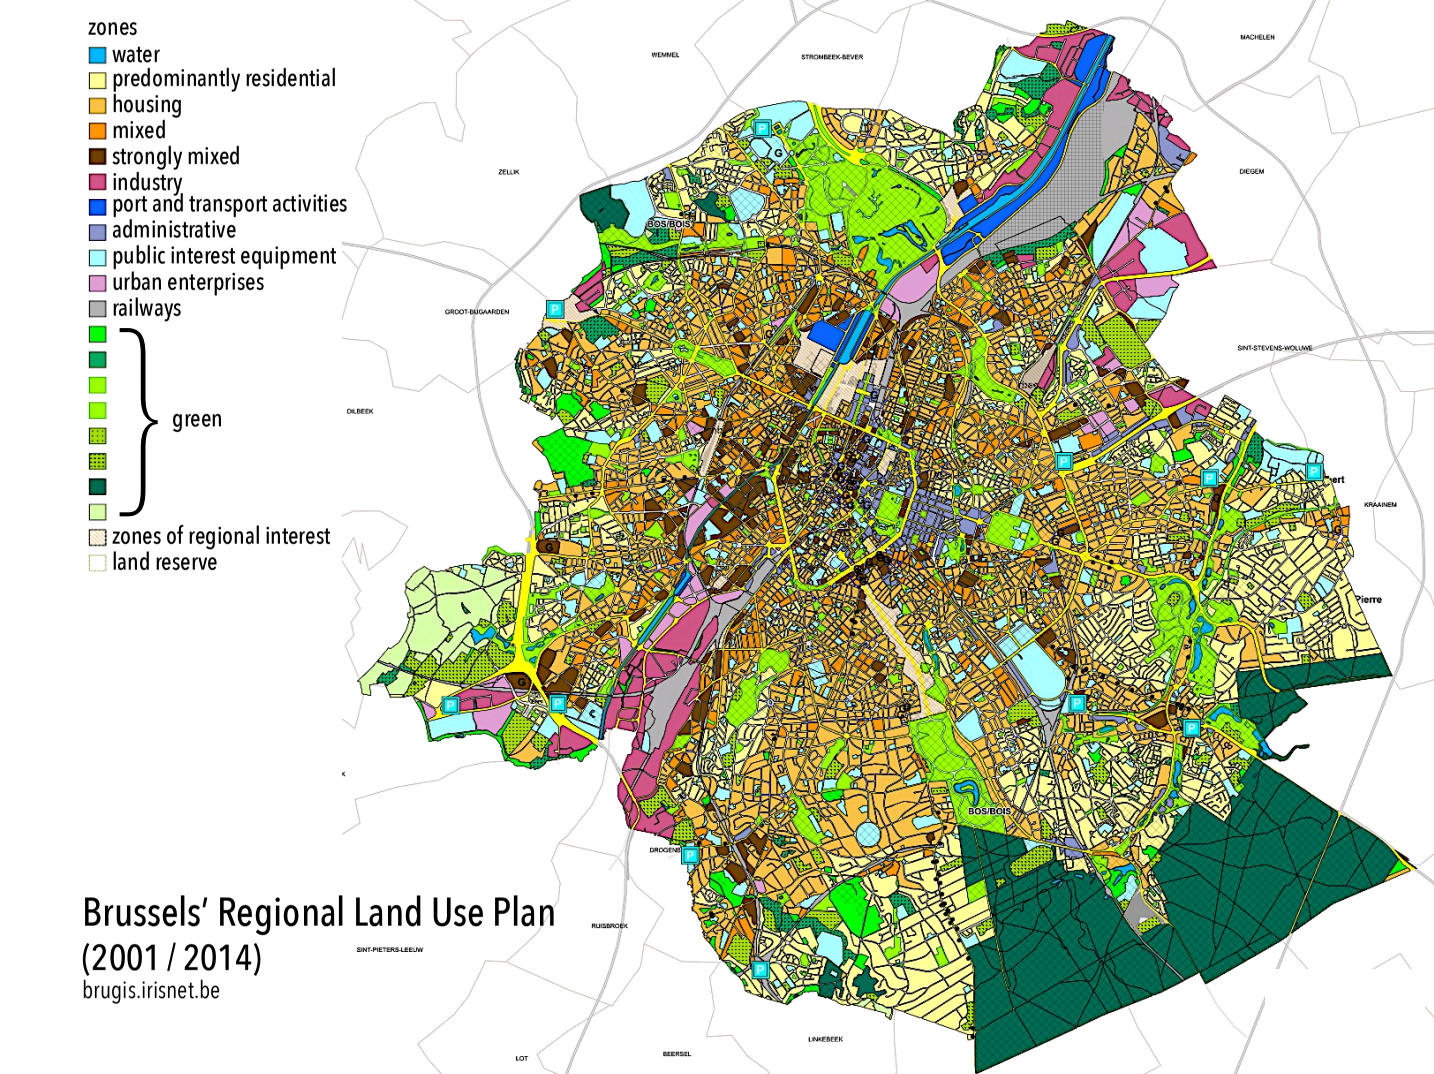
\includegraphics[width=19em]{land_use}
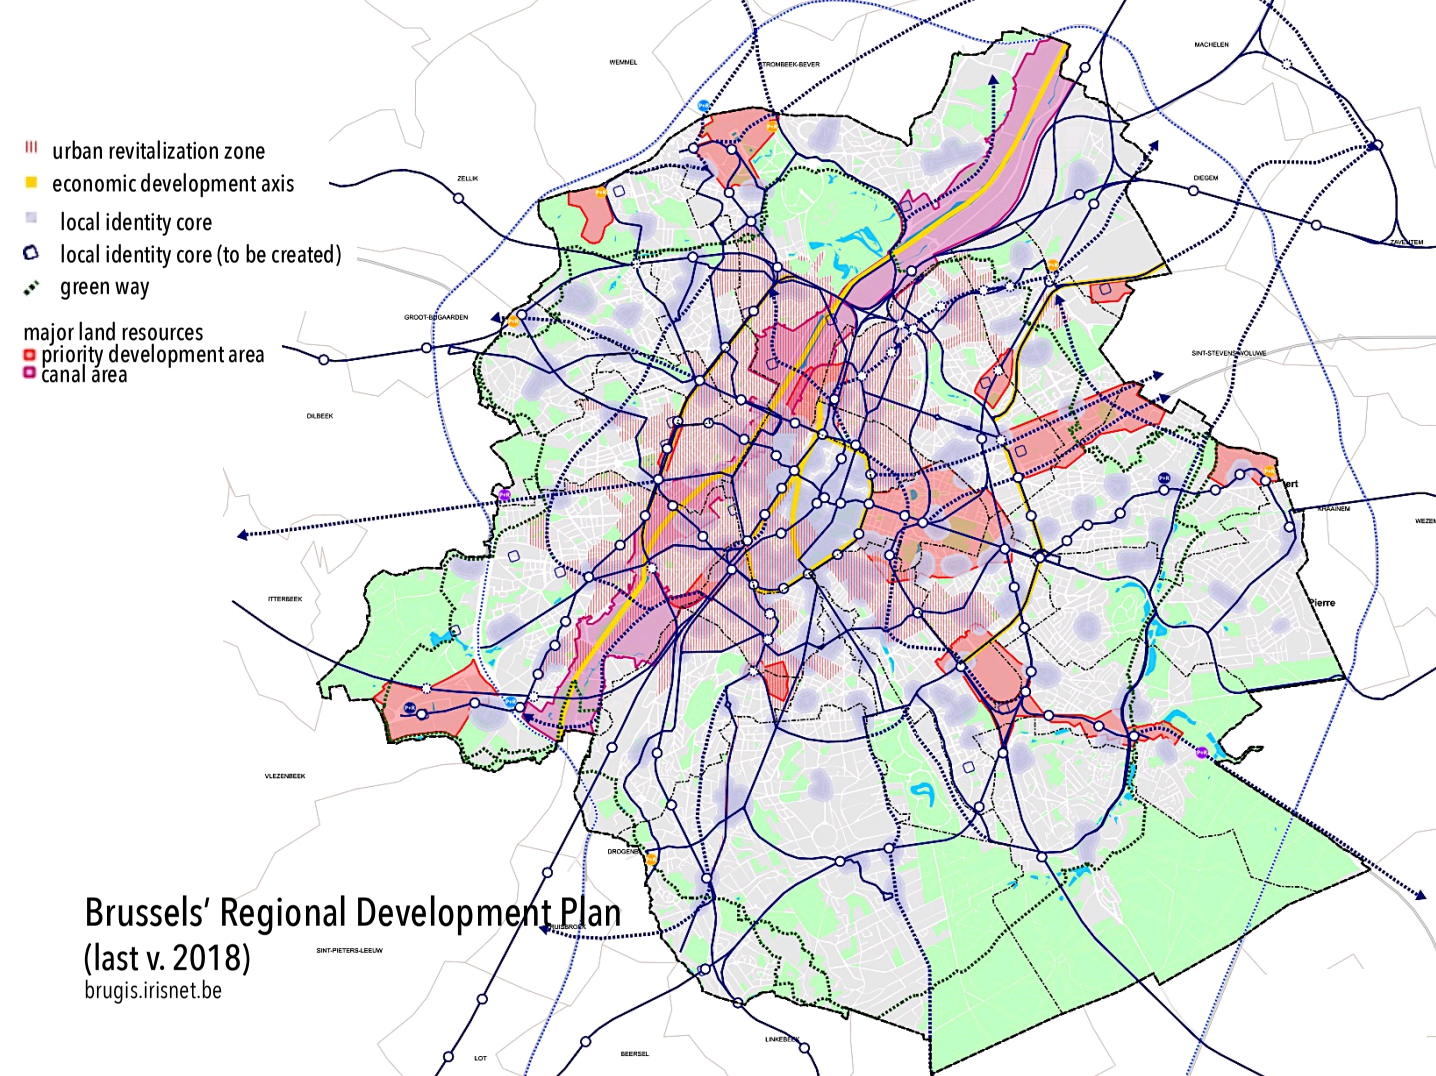
\includegraphics[width=19em]{strategic_plan}
\end{center}

\subsection{Rise of Urban Entrepreneurialism}

\subsubsection{The entrepreneurial script}

What is an entrepreneurial city script? It views the city as a company, in a market environment, which must be competitive.
\url{www.worldbank.org/competitivecities}

\begin{outline}
	\1 A successful city means growth
	\1 Make the city look like a business friendly environment: relax regulation/lower taxes, improve infrastructure, provide incentives, boost city's image...
	\1 There are many blind sports: shared prosperity for all? how so? is this automatic? Being competitive means that some cities are winning, and some are losing. Urban development is not equal. \marginpar{Astana! Not shared prosperity for all, even within the city}
	\1 One recipe does not fit all, because there's a diversity of local contexts. Cities should not all run the same race, and should not all be doing the same thing
	\1 Governments should make the city a friendly and attractive place for business, but should not focus on a single type of business; what about other parts of the economy that make a city, like schools, theatres, hospitals etc. (ULB doesn't have to be attracted to Brussels).
Cities aren't only 'entrepreneurial', and do much more, but competition is usually considered the path to success
\end{outline}

\begin{center}
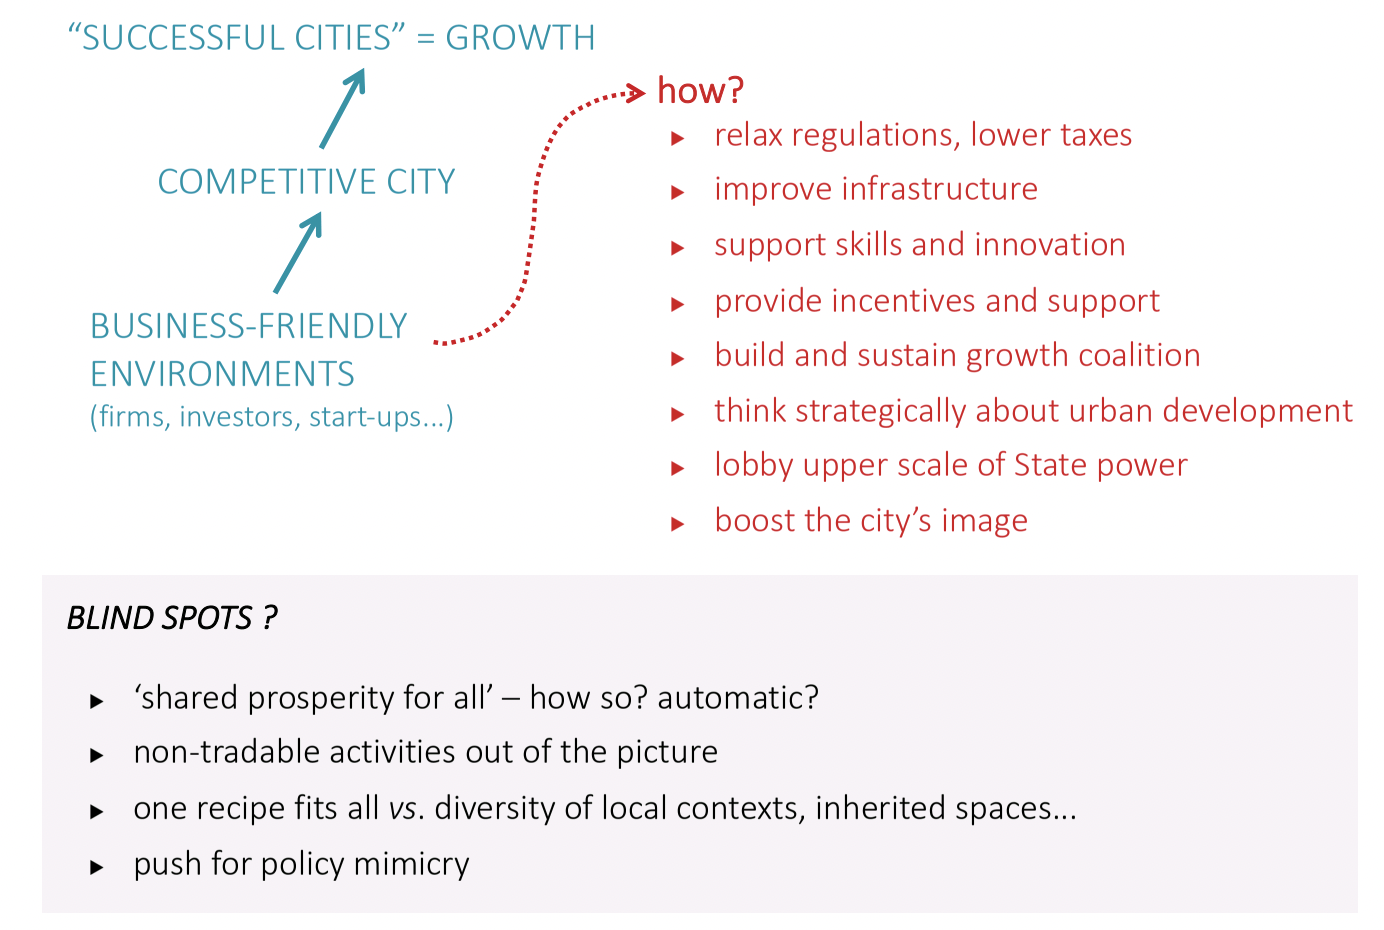
\includegraphics[width=30em]{entrepreneurial_script}
\end{center}

\subsubsection{The entrepreneurial city}

Entrepreneurialism is the mainstream in urban/regional policy. It's often kept outside the space of debate, hailed as ``TINA'',  there is no alternative, and it's a post-colonial condition (Erik Swyngedouw).

The entrepreneurial city focuses on 3 dimensions:
\begin{outline}
	\1 Inter-urban competition: driving the adoption of entrepreneurial stances in urban policies
	\1 Supply-side economics: the overarching development strategy
	\1 Symbolic policies: key and most visible expression 
\end{outline}

\subsubsection{Inter-urban competition}

Inter-urban competition is a cognitive matrix, in which `competition', `entrepreneurialism' as critical concepts. It's a way to take a critical look at evolution of urban governance: cities need to be competitive, otherwise they will decline.

This is not intuitive - how can you imagine that Brussels is in competition with Amsterdam? And that residents, hairdressers, hospitals, etc. in either city, are in competition with their counter parts in another?

David Harvey, 1989, \textit{FromManagerialism to Entrepreneurialism: The Transformation in Urban Governance in Late Capitalism}:

\begin{outline}
	\1 There is a rise of a disposition on the part of public authorities, to govern cities as private corporations in market environments
	\1 Public authorities are taking over attitudes distinctive to market actors (image promotion, risk-taking...)
	\1 There is a generic prioritisation of economic performances over social redistribution
\end{outline}

This is a contrast to the OECD, which has a normative call to urban governments to adopt entrepreneurial approaches as a necessary adaption to an increasing inter-urban competition; ie. ``adapt or lose''.

If competition and entrepreneurialism is not intuitive, where does it come from? 

\begin{outline}
	\1 Rise of `new public management' since 1980s
		\2 An effort to make public administration more business-like and improve the efficiency of public services. It uses competitive forms of resource allocation (eg. project based funding), leading to the \textit{creative destruction of the state}
	\1 Increased trans and intra-national mobility of capital, leading to the \textit{creative destruction of the economy}
		\2 An anticipated consequence of the neoliberal reforms passed since the 1980s, like the liberalisation of capital markets, free-trade agreements, privatisations...
		\2 An example of inter-urban competition is Amazon HQ2\footnote{Amazon asked for cities to bid for their 2nd headquarter after Seattle, promising to create 50k jobs. They had many requests, such as tax breaks and attractive city vibes. Several hundred cities bid, and NYC ended up having to pull out because of push-back from residents}. Inter-urban competition is not natural: cities aren't in competition, but are put in competition with each other by powerful actors.
		\2 The Intensity of inter-urban competition is historical and geographical, and it depends on existing regulatory frameworks
\end{outline}
	
\subsubsection{Supply side economics as development strategy}

The strategy is to invest in the quality of a place, which will bring urban competitiveness, which will bring economic growth, resulting in trickle down effects (activity, jobs, tax returns...), which means more investments in the quality of place.

``Trickle down economics have never worked'' (Biden). This means that instead of bidding for Amazon, the city could fund itself and not wait for Amazon to come in and fix eg., the transit network. The city should be grown ``from the bottom and middle out'', not at the top.

\subsubsection{Symbolic policies}

\textbf{City marketing} is promoting local advantages of a place. This is not a new concept
\textbf{City branding} is new. Can be seen with the fact that all cities now have a logo, but the logo does not say much (or anything) about the city. It's a tool to build a brand, just like for company marketing: it's an advertising techniques applied to cities, aiming to produce a desire, speaking to the heart and feelings, and not to the head, of potential customers. It's building attachment to a place\footnote{eg. I love NY logo} \marginpar{Is there an Astana city brand?}

%%%%%%%%%%%%%%%%%%%%%%%%%%%%%%%%%%%%%%%%%%%%%%%%%%%%%%%%%%%
%																			 LECTURE 5
%%%%%%%%%%%%%%%%%%%%%%%%%%%%%%%%%%%%%%%%%%%%%%%%%%%%%%%%%%%

\section{Culture as Urban Regenerator?}

\subsection{Museums as Political Projects}

Cultural projects have moved centre stage in political agendas, and not only in global cities.
For example, new museums with ambitions of being more than museums, such as regenerating an (urban) area, like Roubaix, Graz. Taking place in second-rate cities would not be possible with an event such as the Olympic games; these could not be situated anywhere else than world cities.

\textbf{Kanal Centre Pompidou:} Centre Pompidou is an arts centre in Paris, and one of the largest art collections in the world.
The site for the Kanal Centre Pompidou is situated in a 1930s Citroen showroom/garage building, along the canal. 
The museum plan is part of an urban policy, beyond the field of culture. 

Branding video: Brussels is branded as the capital of Europe, but Europe is not a nation state and thus doesn't have a capital. Especially not Brussels, which is not one of the most influential cities. The museum is used for urban regeneration, the plan is to bring people together, and make it a social project, but does contemporary art really do that?

The SAU (Société d'Aménagement Urbain) assembles the public and private actors responsible for planning, transforming, managing the site. The estimated budget is 225 million €, and is funded publicly, ie. with tax-payer money.

Thus, museums are ways for policy developers to reach goals beyond the area itself: economic upscaling, building strong international ties.

The question is, \textbf{to what extent can culture act as an urban regenerator, and what are the consequences? Does it work, for whom, and in whose interest?}

\subsection{Culture-led Urban Regeneration}

\subsubsection{Culture-led regeneration script}

1. Invest locally in cultural externalities...

\begin{outline}
	\1 \textbf{Consumption facilities}: flagship museums, large events...
	\1 \textbf{Production facilities}, activities, businesses: turning former industrial sites into art/cultural clusters...
	\1 \textbf{Cultural amenities}: festivals, galleries, public art...
\end{outline}

2. ... and expect a wide range of beneficial impacts

\begin{outline}
	\1 \textbf{Economic}: tourism, jobs, investment, night economy (ie. consumption activities taking place at night)...
	\1 \textbf{Urban}: reinvestment of vacant sites, heritage preservation...
	\1 \textbf{Symbolic}: post-industrial re-branding\footnote{Does Brussels have a strong international image? Its synonymous for the EU, and Brussels is only used to speak of the Commission/Parliament but not of the city itself. Thus, Brussels has a strong image but a very specific one (bureaucratic), and is not the one that the people promoting tourism want.}
	\1 \textbf{Social}: sense of community, civic pride, social cohesion...
\end{outline}

Culture-led urban regeneration is a new concept in the sense that it now features prominently in literature and policy agendas, which was not the case half a century ago. 

\subsubsection{Beyond the script}

There is \textbf{large enthusiasm on the side of policy-makers}, no one is against culture
This enthusiasm is often met with \textbf{perplexity on the side of (critical) scholars}. Studies show that culture-led urban regeneration is `wishful thinking', and in reality the actual benefits are below expectations. The high cost doesn't match the evidence on the consequences of the effort, and the high expectations don't match reality (eg. there aren't as many jobs created).

Thus, \textbf{how do we make sense of the large audience of ``cultural recipes'' to urban (re)development among urban policy makers?}

At first sight, 

\begin{outline}
	\1 There are strong incentives on the part of international institutions
	\1 There's a ``we can do it too'' attitude, and that there is one recipe that fits all; the recipe is not restricted to huge agglomerations, small and medium sized cities can also use it
	\1 Culture is a powerful consensus-making instrument in local politics, no one is against culture
\end{outline}

A step more,
\begin{enumerate}
	\item Shows the power of circulating ``success stories'' proposing accessible ``policy fixes'', with ``mobile policies'' that are easy to copy paste, eg. \textbf{Guggehnheim effect}
	\item Shows the normalisation of culture as an instrument of urban entrepreneurialism, eg.  \textbf{European Capital of Culture}
	\item Shows background influence of the  \textbf{``creative class'' theory}
\end{enumerate}

\subsection{Power of Success Stories}

\subsubsection{The Guggenheim Effect}

The Guggenheim Museum in Bilbao was built in 1997
It has been presented as the success story of culture-led urban development, where Bilbao and Biscay (the region) were `saved' from disinvestment. In the late 20th century, Bilbao was hit with deindustrialisation, and faced political unrest with regards to País Vasco. The Guggenheim effect  was a `renaissance' for Bilbao.

The Guggenheim development was part of a strategic and broader urban regeneration story. Bilbao wanted to transform part of the river bank into an extension of the city centre, and the museum was to be a flagship development amongst other 

The \textbf{objective} was to boost transition from industrial past, to service oriented economy, with focus on tourism and advanced business services (companies, firms, new businesses, service activities, who would relocate from Barcelona/Madrid).

The \textbf{strategy} was to use large public investments in the first place. For the museum, the land was be transferred to the internationally expanding Guggenheim Foundation, \$20 million invested for the name, and \$230 million invested for the construction of the museum. \textit{ie. the Guggenheim was looking for an offshoot location as part of its internationalisation strategy; they made an agreement with the Bilbao/Biscay officials; the region paid for the name and construction of museum.}

For the waterfront area, the former harbour area was to be recycled into an urban neighbourhood to ``work, live and play'', and develop infrastructure works like trams, metro, refurbished public spaces, and a new bridge.

The \textbf{impacts} were

\begin{outline}
	\1 An undeniable tourist boom, with 60\% from abroad
	\1 Poor results in terms of business relocation, and very few companies chose Bilbao over Madrid/Barcelona (ie. large agglomerations)
	\1 A concentration of the culture development budgets into a single project, at the detriment of others
	\1 A quasi-privatisation of urban redevelopment. Who ran the (publicly funded) development? Not the government, but the Bilbao Ria 2000 ltd company, which is controlled by public authorities but with autonomous agency; private actors sign contracts with real estate developers, for new infrastructure; the company is not accountable to the local Parliament for their operations
	\1 Public authorities relying on land valorisation to pay for investments (selling plots, tax returns...), ie. a model of \textbf{Value Capture Finance}, where public projects are financed through monetary valorisation of land resources. This generates a systemic increase of land prices, and the eviction of activities and populations unable to support higher rent values
		\2 It was financed by selling the land owned by public authorities, to private developers; \textit{You sell land with surplus value, it brings you money back, to pay for a museum/other projects; this systemically boosts the land prices; it makes it impossible for the remaining (industrial) activity to stay, because they can't pay the rent anymore; eg. a printing company in the waterfront location cannot pay the rent in the newly attractive, tourism location, compared to a Sheraton}
\end{outline}

\subsection{Culture as Urban Entrepreneurialism}

\subsubsection{European Capital of Culture}

European Capitals of Culture started in 1985 in national capitals (Athens, Florence, Amsterdam, Berlin, Paris), and moved to regional cities starting with Glasgow.

The initial ambition was cultural content for the EEC (European Economic Community). There was the feeling that Europe was missing a cultural project, something to bring people together over something common they had in common. In other words, to depart from a  purely economic project - you can't feel compassion with others over a free-trade agreement. The plan was to showcase what makes people European, in their diversity, with a cultural festival (shows, exhibitions, concerts).

What is European culture? That what makes Europe different from other continent's culture. It's a constant discussion about what it means to be European, beyond free trade agreements.

Between 1986-1989, following Athens, the selected cities were cultural hotspots in Europe. 
1990 was the first time a city without a well established cultural aura was nominated. The reason is that Glasgow's local authorities lobbied and provided funding to organise the event. A year-long campaign ran to promote a post-industrial image of Glasgow.

From 2000 onwards, the ECoC considered a wider audience and more candidate cities. The rules were adapted from a fixed rotation between member states to an intra-national competition. 

Some lessons:
\begin{outline}
	\1 Glasgow 1990 was pioneer of new entrepreneurial template for the ECoC. It launched a new philosophy, from a program to promote urban culture to a program of place promotion. Cities promote themselves (what does the city have to offer) rather than European culture
	\1 There is a concentration of budgets on a selection of places/institutions, at the expense of other places/institutions
	\1 There are uncertain long term impacts: what about the equipments/infrastructure after the event is over? Usually, the number of museum visits drops, ie. momentum falls
\end{outline}

\subsubsection{David Harvey, \textit{The art of rent}}

A wider interpretation of the Guggenheim and ECoC

\subsection{Creative City}

The Creative City claims to be broader and less defined than culture itself: from a \textbf{culture-led} towards a broader \textbf{creativity-led} urban development script

\subsubsection{Creative Class Theory}

Richard Florida, \textit{The Rise fo the Creative Class and How it's transforming work, leisure, community and everyday life} \url{www.creativeclass.com}

Creativity in Florida's terms is much larger than the people who produce `art', there are creative lawyers, traders, engineers... Artists and designers are considered `bohemians' in his model. The Creative Class encompasses circa 30\% of people in the USA.

Florida's arguments:

\begin{outline}
	\1 The presence of the creative class is what makes the urban and regional economies thrive in the post-industrial era
		\2 It has roots in human capital theory: human capital has to be nurtured, developed by the individuals themselves, in order for individuals to be competitive; competitive gains are not made by bringing many workers in to one factory, but instead, by investing in workers to develop their own capacity
	\1 There is a strategic issue: how to attract the creative class to your city? There is a magnetic \textbf{``quality of place'', or ``people's climate''} of a city
		\2 What makes the ``quality of a place'' and attracts the creative class is a series of ``soft'' location factors responsible for ``authenticity'', ``cosmopolitanism'' and ``vibrancy'' (eg. festivals, trendy bars, gay friendly districts, designed public spaces, art events, bike sharing systems, open air swimming pools...). This paints a city as a welcoming, vibrant, cosmopolitan place
\end{outline}
		
The ``creative class theory'' is made of Tolerance, Talents, Technology. Tolerance will attract talent, and talent will bring the technology. 

\begin{outline}
	\1 Tolerance: towards diverse, cosmopolitan individuals
	\1 Talents: what needs to be attracted
	\1 Technology: high tech, modernity
\end{outline}

This is a reversal the conventional strategy of urban/regional development: the creative class (workers) bring firms, and not the other way around. Cities should work to attract individuals rather than businesses.

\subsubsection{Critiques of the Creative Class}

On notions:

\begin{outline}
	\1 \textbf{Creativity} is defined in a very restricted sense, where culture and human creativity are commodified (eg. an old woman painting for her grandkids is not considered creativity)
	\1 \textbf{Class} is not spoken of, it is rather a collection of individuals with `creative' skills and human capital, detached from a wider consideration of social relations. The `creative class' has no consideration of class relation or conflict, and the working class and low-paid workers are barely present in the discussion even though they are part of the infrastructure that supports the lifestyle of the creative class (low paid, highly flexible jobs)
\end{outline}

Empirical limitations: is there evidence for Florida's claims?

\begin{outline}
	\1 ``talent brings firms'' or ''firms bring talents''?
		\2 \textbf{Correlation does not mean causality}: the fact that there is a higher number of gay couples in one city, and at the same time a higher number of people with Bachelor degrees, doesn't mean there is a link between the two
	\1 Are ``creative class'' members really highly mobile individuals, choosing their place of residence and always prone to revise them?	
	\1 Are soft factors really determinant of their location choice?
		\2 ``Accommodating creative knowledge'' study shows that the reason people live in a city, is because of their personal connection/trajectory and hard factors (job opportunity, income levels, infrastructures, education), rather than soft factors (eg. attraction to the city, presence of nature, quality of housing, safety)
\end{outline}

Thus, the ``creative class theory'' is not a theory. But, it's popular amongst policy makers because it legitimates entrepreneurial urban development, that focuses on improving quality of life (but for who?) and anticipating trickle-down effects, contra investment in local welfare. The creative class boosts gentrification trends, possibly leading to displacement of many ``creatives''.

\subsection{Alternatives to Creative Class Theory}

\begin{outline}
	\1 Artivism\footnote{Hamburg artists' initiative who refused to brand Hamburg as a ``pulsating capital'', which offers a ``stimulating atmosphere and the best opportunities for creatives of all stripes''}
	\1 Pay closer attention to the actually very diverse landscape of art and cultural practices and less to success-stories. The former are usually below the radar of policy makers, but have an actual impact on the lives of urban dwellers, contrary to success-stories which simply aim to attract new comers and not address existing residents' welfare
	\1 Non-entrepreneurial cultural projects are possible:
		\2 Detach cultural goals from place competitiveness and attractiveness concerns
		\2 Consider how arts, culture, creativity, are vehicles for emancipation and NOT place-marketing 
\end{outline}


%%%%%%%%%%%%%%%%%%%%%%%%%%%%%%%%%%%%%%%%%%%%%%%%%%%%%%%%%%%
%																			 LECTURE 6
%%%%%%%%%%%%%%%%%%%%%%%%%%%%%%%%%%%%%%%%%%%%%%%%%%%%%%%%%%%

\section{Everyday Life}

\section{(Contra) Gentrification}

Gentrification can be used as a lens to articulate the spatial practices of capital, and territorial regulations.

Gentrification has gained an audience in academia, and circulates beyond. It's rare that academic terms do this. You can find gentrification in comic books, sports, popular culture, and is appropriated by grass roots movements who try to oppose and contest urban renewal programs.

Gentrification literature has taken off significantly since mid 2000s, and is now a specialisation within urban studies. The field is now international, and cities on all continents are studied.

\subsection{Origins of the concept}

Ruth Glass, 1912-1990, German born sociologist who fled to England. Founder of gentrification.
Researched urban change in Central London and coined the term `gentrification'\footnote{Ruth Glass, \textit{London: aspects of change}, 1964}

\begin{outline}
	\1 \textbf{A residential process}: dwelling by dwelling rehabilitation of existing housing units leading to the gradual displacement of incumbent residents
	\1 \textbf{A sporadic and limited process}: restricted to certain neighbourhoods, other authors especially in the US had the same observations
	\1 \textbf{An unusual direction of neighbourhood change}: depicts a direction of urban change that is the opposite of the Chicago School model, that is middle classes moving into the city centres; thus, it challenges the dominant theory
	\1 \textbf{Is more than a descriptor of a particular process of urban change}: the name has a British origin, `gentry' is a purely British term, criticises those who have money and power but did nothing to acquire it
	\1 $\Rightarrow$ \textbf{A critical intent built into the etymology}: naming a class remaking of urban space and its associated dispossessions
	\1 $\Rightarrow$ \textbf{A politically loaded term}: unlike ``urban revitalisation'', ``regeneration'', ``renaissance'', ``renewal'', ``upgrading'', ``social mixing''...
\end{outline}

\subsection{Variegated gentrifications}

Internationalisation of gentrification research in early 2000s, deviates from Glass' initial definition.

\begin{outline}
	\1 Rural gentrification
		\2 Works are mostly in Great Britain, USA, France
		\2 Middle to upper class remaking of some rural areas endowed with specific amenities, eg. architecture, climate, National Park, accessibility from metropolitan areas, etc.
	\1 Transnational gentrification
		\2 Change is triggered by the influx of visitors (tourists, lifestyle migrants, digital nomads, retirees, expats)
		\2 Process accelerated by the rise of rental platforms like Airbnb, and place promotion by the cities
		\2 Eg. the Gòtic neighbourhood of Barcelona: from 1998 to 2016, drastic increase in young adults (25-49) from outside Spain, predominantly from Europe, South America, Asia
	\1 Marginal gentrification
		\2 Typically young adults, educated, single or unmarried without children, starting professional career path
		\2 Turnover on the private rental market, rather than rental-to-?; ie. renters replacing other renters, `rental gentrification'
		\2 Eg. Mile End, Montreal
	\1 New-build gentrification
		\2 Looking not at places that are reconstructed, but at new developments
		\2 Eg. Tour \& Taxis
	\1 Mega-gentrification
		\2 A XXL version of new-build gentrification, mostly in the global South
		\2 Wholesale clearance of large, densely-built workers' compounds (incl. slums) or older industrial complexes to make room new-build projects lying far beyond the reach of original residents
		\2 Radical transformation within a highly compressed time scale; in Beijing and Seoul, for the Olympic games
		\2 Eg. China, South Korea
\end{outline}

This is a non-exhaustive list... retail gentrification, productive gentrification, super gentrification, tourist gentrification, slum gentrification, etc.

\subsection{Gentrification as a generic concept}

What makes a good concept? Should a concept be limited to a time space context, or, generic in order to bring together realities that may be distinct at first sight but share a common skeleton and that can be researched by many researchers with a diversity of backgrounds? In the case of gentrification, generalisation makes more sense.

\begin{outline}
	\1 Gentrification is now rooted in the political economic of contemporary capitalism\footnote{Lees, Shin, López-Morales \textit{Planetary Gentrification}, 2017}
	\1 Crucial role of State actors
	\1 $\Rightarrow$ Planetarisation of state and capital gentrification strategies. It does not mean that gentrification is taking place everywhere at all time, but that policies that implicitly encourage gentrification are proliferating worldwide
\end{outline}

Mathieu's 
\begin{outline}
	\1 Working definition: Any form of reconfiguration of popular spaces to the advantage of socially advantaged groups, resulting in various forms of dispossession of ordinary users of these spaces
	\1 Purpose: pointing the power conferred by an affiliation to a dominant social position to reshape working-class space to one's own advantage
	\1 $\Rightarrow$ Gentrification is about:
		\2 A form of class power over space
		\2 A power over the production of space, to transform and not to access currently existing space
		\2 A power to remake popular spaces: urban or rural, residential, leisure or productive. It is an upgrading of a space where upper-classes are not dominant, where they can take the space and use it to their advantage
		\2 $\Rightarrow$ using social power to produce space, and the social consequences of this, like dispossessions
\end{outline}

How do these social powers that transform/reshape popular space, work?

\begin{outline}
	\1 Movement of capital at the intra-urban scale; investments to parts of the city that were neglected or not attractive to investors in previous decades
		\2 \textbf{Rent gap theory}: understanding why investors move to neighbourhoods that they have ignored for decades
	\1 State support to gentrification dynamics
		\2 State led gentrification
	\1 Middle class appropriation: 
		\2 Material and symbolic makeover of popular spaces
	\1 $\Rightarrow$ a power exercised through \textbf{system effects}, without centralised coordination
\end{outline}

Dispossession as a constituent of this power over space

\subsubsection{Rent gap theory}

Neil Smith, \textit{Toward a theory of gentrification: A back to the city movement by capital, not people}, 1979

Why do investors start investing in neighbourhoods which they ignored for decades? What changed? $\rightarrow$ rent gap theory

Rent gap theory: the difference between the capitalised ground rent under present use, and the potential ground rent under `highest and best' market use

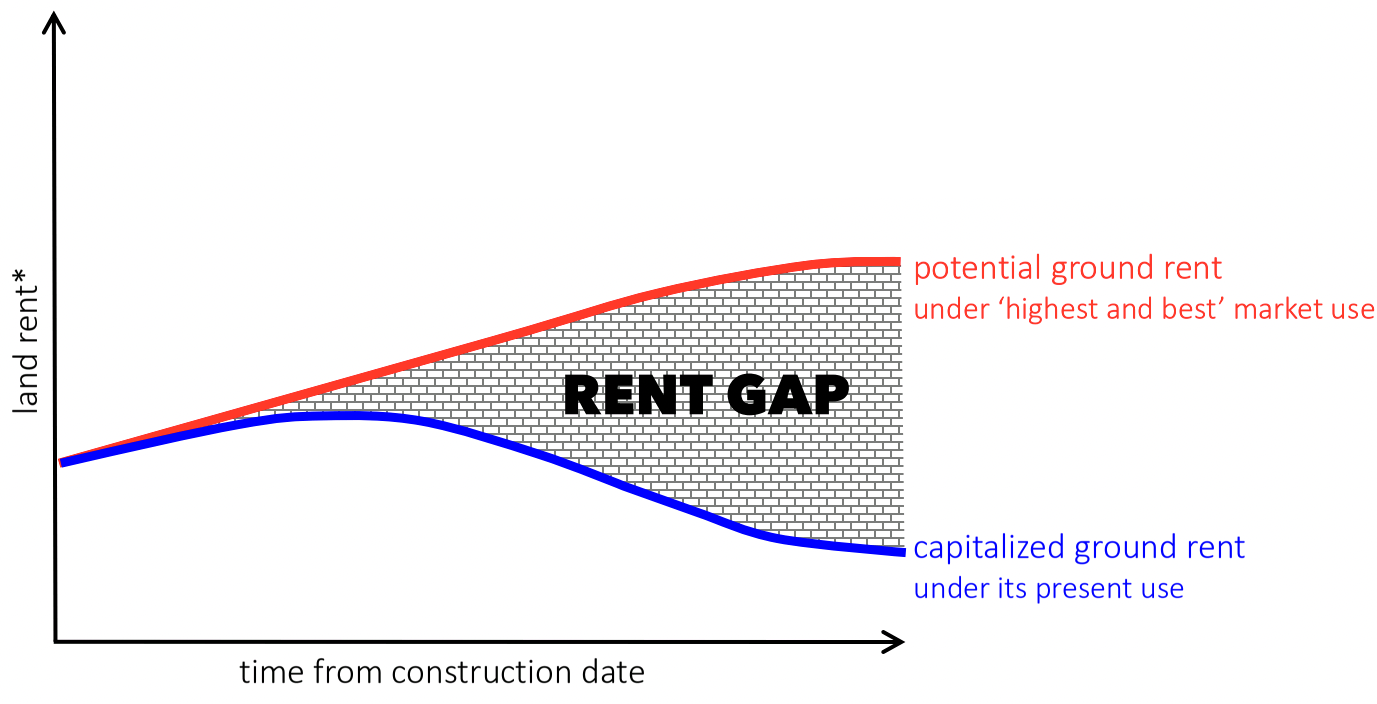
\includegraphics[width=\textwidth]{rent_gap_theory}

Rent gap theory has been rejuvinated by financialisation, which gives an extra boost to rent-gap mechanism as a profit-making strategy

eg. Airbnb from charing economy toward investment niche for rent-seeking capital.

There is nothing `automatic' about the rent gap. It is necessary for the existing rent to be lower than the potential rent, but it is not enough. It also takes some form of \textbf{collective social action} on the neighbourhood level to actually bring the investment, to produce or close a rent gap, bringing together developers, mortgage lenders, entrepreneurs, and State institutions

\subsubsection{State-led gentrification}

Another deviation from Glass' initial formulation: from agent-led process (households or developers) to state led projects, and from small-scale initiatives to large-scale programmes

Gentrification is no longer about bottom-up, small scale initiatives, and small actors investing money in land, but a part of the political economy of urban development, involving a combination of diverse policies and state interventions, with no single `gentrification policy'.

Type of state interventions include:

\begin{outline}
	\1 Material interventions: installing new equipment
	\1 Regulatory interventions: allowing more floors to be built on the same plot of land
	\1 Symbolic interventions: city marketing campaigns, place promotion
\end{outline}

In Brussels' canal area, state interventions look like: new equipments, changing regulations, symbolic effort to rebrand canal into attractive residential area for people who can choose where they live because they have enough money to do so\marginpar{Photo essay}
Policy makers will say ``we're not pushing gentrification, we are pushing social mix'', but de facto we can see that gentrification is happening. $\rightarrow$ gentrification by stealth

Gentrification has turned into a strategic option of urban policies, in many different contexts, that can compete or be combined with other policies, in the name of social cohesion, social mixing, creative cities, etc. but never in the name of `gentrification'. The policies create the environment in which gentrification occurs.

\subsubsection{Material and symbolic makeover of popular spaces}

The real gentrifier is not the hipster, but the capital and the state acting together to make gentrification possible, to reinvest in or push out populations in favour of others. The people who are the gentrifiers, are not doing it consciously. They are not trying to gentrify the neighbourhoods, but nevertheless they take part in the gentrification process, even without an intention to do explicitly.

\begin{outline}
	\1 Adjustment of various material and symbolic characteristics of working class neighbourhoods to a new set of middle-class norms
	\1 Diverse expressions, incl. patronising new retail landscapes made of fashion/home decoration boutiques, `trendy' cafes/restaurants, art galleries, ie. retail gentrification
	\1 New class identity\footnote{Ley, \textit{The new middle class and the remaking of the central city}, 1997}
		\2 Gentrification is a process of class constitution through urban change
		\2 Appropriating new landscapes of ``authentic'' or ``alternative'' consumption as a way to forge a distinctive social identity, distinct from the working class, traditional bourgeoisie, and suburban middle class
	\1 Feminist insights 1980-1990s: preference for central-city living over suburbia as an expression of the breakdown of the patriarchal household, and of the rise of more egalitarian dual-earner household arrangements. But for most women gentrification is not emancipatory
\end{outline}

\subsection{Dispossessions}

Dispossession is built into the concept of gentrification. Stories of gentrification are also stories of dispossession, but of different forms and mechanisms: the story is not the same everywhere.

\begin{outline}
	\1 Direct displacement
		\2 Economic motives
		\2 Physical motives
		\2 Legal motives
	\1 Indirect/exclusionary displacement
		\2 Those who are excluded are not necessarily the displaced, but those who are not allowed in
	\1 Neighbourhood resource displacement: losing a sense of place, a supportive local environment, neighbours moved out, food shops are replaced by art galleries
		\2 \textbf{Losing a sense of place} :you need a place to feel at home, where you are accepted, and not simply a roof and a bed
	\1 Community displacement
\end{outline}

Nearly impossible to put a figure on the number of people who are displaced. This is problematic for those who demand figures to prove something exists. Even for direct displacements, where people are asked to move, it is hard to measure displacement - you need to keep up with their new addresses. 

\subsection{Contra gentrification}

Gentrification as an ``unstoppable tidal wave'' of profit seeking reinvestments and associated dispossession sweeping across passive neighbourhoods.

However, you can find places where gentrification is occurring but is resisted, slowed down, or opposed by local elements such as the population, or local activities. 

Why do some places not gentrify?

What and who runs \textit{contra} gentrification?

Because of different types of \textbf{resistance}

\textbf{Resistance is not resilience}.
Resilience is how space adapts to change from external forces that are left unquestioned.
Resistance is for what holds existing socio-spatial configurations in their present state.

Resistance to gentrification takes different forms
\begin{outline}
	\1 Collective mobilisation: urban social movements, urban struggles
	\1 Claiming the right to stay put, to maintain existing uses of the space re housing, work, retail, public spaces, ie. an improvement and not a replacement
	\1 
	\1 $\Rightarrow$ resistance for oneself, through mobilisation, that is highly politicised
	\1 ``Ordinary'', ``everyday'' resistances: much of the politics of subordinate
		\2 $\Rightarrow$ resistance in itself
\end{outline}

Public/private forces backing gentrification are powerful, but gentrification processes do not roll out on blank pages. We mustn't underestimate the power of other forces. As long as popular neighbourhoods remain inhabited, lived or appropriated, existing places aren't simply up for grabs.

%%%%%%%%%%%%%%%%%%%%%%%%%%%%%%%%%%%%%%%%%%%%%%%%%%%%%%%%%%% 
%																			 LECTURE 7
%%%%%%%%%%%%%%%%%%%%%%%%%%%%%%%%%%%%%%%%%%%%%%%%%%%%%%%%%%%

\section{Ordinary Urbanisations}

\textit{tldr; how inhabitants produce space, alongside capital and state actors; inhabitants contribute to the production of space in their own right, through their ordinary uses of urban space and their spatial practices as city users}

The inhabitants of a city aren't only the residents, but all people who use the city. 

For example, Las Ramblas: how are these kinds of spaces produced? They are produced by businesses, shops, tourists, transport companies who bring people to Barcelona, city marketing campaigns to attract tourists in view of development of the local economy.
Tourists themselves are involved in the production of this space, both symbolically (the space exists because of tourist demand) and physically (tourists make the space by being in it). The shops and the people (predominantly tourists) would not be there, if it weren't for tourism.

In contrast, there is another category of people who use the space for living purposes: residents. There is a conflict between the residents, and the tourists; those who sleep at night, and those who live at night. 

Thus, there are \textbf{conflicting ways to use space}, and through ordinary uses of space, us city users have a (collective) role in the production this space.

\subsection{Learning from above and from below}

Ananya speaks about the importance of grassroots, informal, ``from below'' movements and concepts regarding inhabitants and the city.

``Urban theory has long been concerned with the ways in which the poor and marginalised act in the face of power. However, it has been better able to explain acts of power than acts of resistance, as in concepts of growth machines, political regimes of redevelopment, modes of regulation, and urban entrepreneurialism. The `Third World' literature on informality is a treasure-trove of conceptual work on the `grassroots' of the city, and is thus able to expand considerably the analysis of `urban politics' or `metropolitics''' - Ananya Roy, \textit{The 21st century metropolis: New Geographies of Theory}, 2009. 

\textbf{Learning from above} is the urban political economy that researches cities and urban change from the perspective of the State. 
\textbf{Learning from below} is coming from the perspective of the governed, rather than from the perspective of those in the public/private governing seats.

\subsection{Ordinary cities}

Jennifer Robinson, \textit{Ordinary Cities}, 2006.

Many cities are left off the map, as a consequence of neoliberal globalisation (they are on the periphery of the financial networks and information flows). Hence, they are implicitly deemed places from which there is nothing to learn.

Think about global cities: Africa has only a handful of cities represented on the GaWC heuristics map. Instead the majority are concentrated in Western Europe, North America, and east Asia (China, Japan). This global cities map excludes very large cities. Global cities promote economic relations, with global reach, and ``prioritise certain prominent sectors of the global economy for development and investment''.

To escape this trap, Robinson proposes to look at \textit{all} cities as `ordinary', and not as a binary `global or invisible'. This is a heuristic proposal, and not a call for completing the map of global cities by adding a new category to the same map. Rather, to create a new map where all cities are allowed to be `ordinary', including NYC, London and Tokyo. 

Ordinary cities focus on other realities of the city. They call for \textbf{cosmopolitanising or provincialising} cities, to theorise, (re-)build concepts, and take inspiration from a wider range of cities and not just the Global North cities. 

Ordinary cities are also the foundation for \textbf{post-colonial urban studies}. The objective is to:

\begin{outline}
	\1 Develop urban theories rooted in and informed by non-Western experiences of urbanisation
	\1 Theorises ``off the map'' places, notably in the global South
	\1 Pay more attention to grassroots, everyday, informal, DIY, etc. dimensions of urbanisations
	\1 Pay more attention for the everyday lives of the urban poor, eg. in favelas, townships, slums, geçekondu
\end{outline}

\subsubsection{Epistemologies of the South}

An epistemological proposal: \textbf{how do we learn and produce knowledge, by looking at what?}

Boaventura de Sousa Santos, \textit{Epistemologies of the South, Justice against Epistemicide}, 2014.

The South is ``a metaphor for the human suffering caused by capitalism and colonialism on the global level, as well as for the resistance to overcoming or minimising such suffering. It is, therefore, an anti-capitalist, anti-colonialist, anti-patriarchal, and anti-imperialist South. It is a South that also exists in the geographic North (Europe and North America), in the form of excluded, silenced and marginalised populations, such as undocumented immigrants, the unemployed, ethnic or religious minorities, and victims of sexism, homophobia, racism and islamophobia.''

There are multiple notions in line with the call for post-colonial urban studies: subaltern urbanism, occupancy urbanism, popular urbanisation, peripheral urbanisation, insurgent citizenship, popular centrality, etc.

\subsection{Subaltern urbanism}

Ananya Roy, \textit{The 21st Century Metropolis: New Geographies of Theory}, 2009.

We need to contest the inherited location of urban theoretical work, which has been done predominantly in the centre of the colonial power rather than in colonised country. In the 21st century, the fastest growing cities are in the global South.

The argument is about the \textbf{situatedness} of urban theory. This does not mean that theories are not applicable to contexts outside of the ones they were created, but to acknowledge that the content of theory depends on where it is elaborated, because theorists think differently when paying attention to urban transformations in the South/North.

The point is to study cities differently, starting from cities in the global South, to get a different grip on urban reality. It isn't to study global South cities \textit{instead of} global North cities, but to start from a different place, because \textbf{any city can be a place for theory-making}.

\subsubsection{Urban Informality}

Not a set of deviant or illegal practices, but a mode of urbanisation, an organic logic, a system of norms that governs the process of urban transformation. 

It can take \textbf{different forms} like squatter settlements at the rural and urban interface, or elite zones.
The main criteria is the the \textbf{distance from formal spatial planning rules or land regulations}.
Informality is not just about the urban poor, but a \textbf{mode of urbanisation} that takes distance from urban (planning) rules and regulations.

Informality is a key dimension of subaltern urbanism.

Examples:

Popular settlements on the fringes of \textbf{Mexico City}; the city is fast expanding, and most of the metropolitan expansion is being driven by informal urbanisation. Producing knowledge first in the global South, and let this concept travel.

\textbf{Cureghem}: informal/illegal street vendors near metro stations, informal housing practices through illegal subletting and slum lords, formal/informal Sunday markets, Rue Heyvart street second hand car negotiations taking place on the street

Master Plan PAD Heyvart: linear park cutting through neighbourhood, forcing garages to move; part of the redevelopment of the canal, to attract startups and business; idea is to transform the abattoir (and more), to have activities more in line with the aspirations of the new middle class rather than the the aspirations of those who already live there\marginpar{Photo essay Porte de Ninove}. Thus, Cureghem is a space produced both from above and from below, notably by inhabitants in diverse \textbf{subaltern} positions developing and relying on informal practices.

Narrow conceptions of informality as illegality, or nuisances, ignore the whole set of issues of livelihoods embedded in the communities, such as social networks, access to jobs or housing, community building,... and give credit to gentrification projects. 

Urban informality is not outside the scope of capital, but is an ancillary part of the formal markets, eg. food, second hand cars, housing.

Urban informality is not outside the scope of the State: surveillance, tacit tolerance, repression. The informal negotiations on Rue Heyvart take place right in front of a police station.

\subsection{Popular urbanisation}

A recent (2020) proposal.

A collective process in the production of space. Driven by the initiative, engagement and labour of the people, usually accompanied by strong social and political mobilisation.

It reveals the \textbf{collective} agency of the population in the production of space, through collective experiences, including mobilisations (eg. claiming land, getting access to services that are denied/not offered by public or private institutions).

Example: \textbf{Geçekondu, Turkey}

Literally means ``settling at night'', geçekondus are originally informal settlements built overnight by rural-to-urban immigrants, on illegally occupied land. The term now includes diverse kinds of informal settlements.

Built from the bottom up, with the absence of the formal market in the face of the amount of people arriving to the city. Migrants doing the job by themselves, for themselves, is easier for the State, and is a cheaper way to provide housing.
Thus, industrialists and state agencies are happy for migrants to do what they can, especially because the former can keep their wages low.

Towards a post-geçekondu city: using earthquakes as argument for destruction and reconstruction of dwellings, a justification for `cleaning' the place by forcing people to sell their homes or face expropriation... although one of the towers that was built anew collapsed in an earthquake in 201?, reinforcing the idea that the destruction/construction is not to protect the population from earthquakes.

\subsubsection{The city seen from below}

Rosa Bonheur, \textit{La ville vue d'en bas}, 2019.

Roubaix is an example of a shrinking city, hit by deindustrialisation. By contrast, in the 19th century Roubaix was a `Manchester' with a strong industrial textile production, ``la ville aux mille cheminées''. 

In an attempt to attract people to Roubaix, the municipality purchased (rundown) houses and proposed to sell them for 1€, and leave the renovation responsibility to the buyer. But, selling houses at 1€ depreciates the value of the houses next door, and thus was not really efficient. But, it shows that Roubaix is a place where renewal programs were implemented to try to reinvigorate the city. For example, they had subsidies for attracting companies, middle class neighbourhoods, urban garden initiatives, etc.

Popular urbanisation research realised that people who are said to `do nothing', like the unemployed, inactive, on welfare, etc. actually work hard in conditions they have not chosen for themselves and with levels of income that keeps them in a state of deprivation. Their work is referred to as \textbf{subsistence work}. This includes:

\begin{outline}
	\1 Producing some goods or services at home, and selling them informally, eg. by putting signs in windows
	\1 Low-budget self-renovation of housing
	\1 Shopping works: organisation of mobilities to get decent food, clothing, equipment, at a low cost; people organising themselves to travel long distances to get resources, for example travelling in one car from Lille to Cureghem to buy cheap meat from the market for multiple families; sharing resources
	\1 Paper works: close monitoring of administrative statuses to get access to/not lose welfare rights
	\1 Economic activities that provide income and meet local, low=budget demands; eg. street car mechanics
\end{outline}

Subsistence work is \textbf{spatial} insofar as it relies on spatial configurations that make it possible for the work to exist, and it helps to reproduce these spaces.

\[\textbf{subsistence work $\leftrightarrow$ popular centrality}\]

\subsubsection{Popular centrality}

A resourceful space, a space made by and for those who are using it. It is a resource in the sense that it is constantly produced and consumed by those involved, in a relational exchange.

Cureghem as a popular centrality: a place where people congregate and meet on a weekly basis, informally; a place for people to find others with the same culture; a multi-resource space (shopping work, economic activities, social contacts, mutual help, reassurance...) (re) produced for and by working-class populations.

Breaking down popular centrality:

\begin{outline}
	\1 \textbf{Popular}: a set of resourceful spaces made for and by populations in socially-dominated positions.
	\1 \textbf{Centrality}: those spaces are absolutely central to the daily lives of the populations using it. Contrast with the planning documents which look like peripheral neighbourhoods that need to be reconnected to the city centre; But if you look at it from below, this is false. There is a strong community and life happening in these neighbourhoods, that do not need any connection to the city centres.\marginpar{Photo essay: porte de Ninove is embedded in a neighbourhood that has popular centrality, yet developments targeting middle class are being developed}
\end{outline}

Popular centrality is a \textbf{resistance space}, and an explication for how certain spaces resist gentrification.

\subsubsection{Resisting gentrification}

Marolles, Bruxelles: 

\begin{outline}
	\1 A neighbourhood next to Cureghem, the poorest statistically in terms of median income per households, with clear gentrification pressure. Is this a paradox? Walking through Marolles, there are trendy shops, cafes, galleries, efforts by authorities to brand Marolles as a street art neighbourhood, launched by an association of upscale shop keepers
	\1 Marolles is 28.7\% social housing, compared to 7.2\% in the Brussels region: this allows low income households to stay in the Marolles; shops can exist alongside the social housing
	\1 Marolles flea market (including professionals), Place du jeux de balle, taking place every morning. A space of intense sociability and economic action, a multi-purpose space, a space of popular centrality
	\1 Successful protest against the parking project in the Marolles, which would have replaced the market with a parking lot
\end{outline}

The flea market is used as a promotion for the city, by the city. Production from below can produce resistance spaces.


Rather than an `outside', the production of popular centralities is fully inscribed in the logics of unequal spatial development. It is because capital has withdrawn from cities like Roubaix, and because urban policies are turning away from the needs of the working classes, that the subsistence work of their inhabitants has a strong impact on a local space.

``The city seen from below'' is not a call to disregard the structural forces shaping urban spaces ``from above'', but to articulate them to social forces acting ``from below''.

%%%%%%%%%%%%%%%%%%%%%%%%%%%%%%%%%%%%%%%%%%%%%%%%%%%%%%%%%%% 
%																			LECTURE 8
%%%%%%%%%%%%%%%%%%%%%%%%%%%%%%%%%%%%%%%%%%%%%%%%%%%%%%%%%%%

\section{On Urban Alternatives}
\textit{December 16th 2021, with Wojciech Kebłowski}

Everyday life $\rightarrow$ gentrification studies, post-colonial urban theory; N. Smith, J. Robinson, A. Roy

\subsection{Situating urban alternatives in the class structure}

\textbf{Market led urbanism}: commodification, growth, accumulation, production and maximisation of economic values through the production of space (eg. real estate)

\textbf{State-led urbanism}: development and control of spatial arrangement for the sake of national territorial development, attached to some definition of justice or legality

\textbf{Popular urbanism}: popular, collective agency, through mobilisations and uses of urban space, for the sake of livelihood, habitat and community building

The \textbf{neoliberal city} can be situated as the alliance of market-led and state-led urbanism.
Urbanisation of neoliberalism, and neoliberalisation of urbanism.

It interacts with urbanisation from below, through processes of disinvestments and dispossession of \textbf{ordinary urbanisation}, and its resistance to forces of the neoliberal city.

\textbf{Urban alternatives} as initiatives in the production of space, at a distance from market-led rationalities (complete opposite) and of state-led urbanisation, but closer to popular urbanisation.

\subsection{Urban alternatives}

New wave of political imagination and praxis in urban governance, economies, transport, housing, public spaces,...

And different politico-philosophical backgrounds: ecologism, feminism, social-democracy, community organising, autonomy, indeginism, libertarianism,...

There are many diverse initiatives like community land trusts and fare-free public transport: transition town, post-carbon cities, urban greening, urban agriculture, local exchange systems/currencies, community-based economies, free shops, circular economies, bike repair, temporary occupations, squats, participatory budgeting, citizen assemblies, community planning, tactical urbanism, housing co-ops,...

Recurring characteristics:

\begin{outline}
	\1 Initiatives coming from the bottom-up: grassroots, citizen-led
		\2 Community organisations or citizens collectives as driving forces
		\2 Not excluding relationships with or support from State authorities
	\1 Initiatives bear an alternative value systems, 
		\2 Distanced from market and growth rationalities, they are non-for-profit
		\2 Distanced from mainstream neoliberal approach to urban politics: addressing head-on the problems faced by inhabitants, rather than via indirect or anticipated `trickle-down' effects (eg. investing directly in social housing rather than businesses that may later indirectly bring some money in to the neighbourhood)
	\1 Generic purpose  of alleviating ?
\end{outline}

\subsection{Community Land Trusts, CLT}

Between state-led housing development and popular urbanism

The land on top of which CLT buildings are constructed is taken out of the market logic, forever, and the cost of the housing is reduced because the price of the land is not included (and will never be).

\begin{outline}
	\1 A non-profit, membership-based organisation chartered to hold and manage a piece of land as a trust on behalf of a given community
	\1 Historic roots in planned communities on leased land (eg. UK garden city movement, Israelis moshav village communities, India's village land trusts)
	\1 First modern-day CLTs created in the US rural south in 1960s, typically to secure long-term access to farmland for African-American farmers
	\1 First urban CLTs in USA in 1980s, in Vermont, in response to inflating housing prices in the city; financial support from local authorities (mayor Bernie Sanders)
	\1 First CLTs outside US and Canada are in the UK, and in continental Europe, Belgium (2012)\marginpar{CLT in Porte de Ninove? see cltb.be}
\end{outline}

\subsubsection{Zooming out: a critical perspective}

\begin{outline}
	\1 At the same time that the government is supporting CLT production, they show increasingly limited ambitions in the field of social housing production
	\1 Residualisation of social housing: publicly subsidised rental housing conceived of only a safety new for lowest income groups; public authorities pushing CLTs but an the other hand being too slow in producing social housing (where everything, the building and the land, is out of the market)
	\1 Regarding urban policies:
		\2 CLTs are developed in areas otherwise targeted by urban `revitalisation' programmes aimed at increasing place attractiveness towards investors and the middle class (eg. the canal project)
\end{outline}

\subsubsection{Critical lessons on urban alternatives}

\begin{outline}
	\1 An alternative label is not in itself a gurantee of immunity against inclusion in policy repertoire, otherwise dominated by neoliberal mainstream; possible instrumentalisation for ``alter-washing'' purposes
	\1 Alternatives are niches, and still have to play with the non-alternative system(s)
	\1 $\Rightarrow$ so to what extent are existing alternatives, really alternative? A proposed conditionality:
		\2 1. a subversion of, or clear challenge to the mainstream `neoliberal cities'
		\2 2. a macro ambition, aiming at changes for the many
	\1 CLT in Brussels today
		\2 1. Yes, to some extent, an obstacle to property speculation
		\2 2. No, absence of `scaling up' perspectives as housing policy; ie. missing a wider alternative politics of the city writ large
\end{outline}

\subsubsection{Right to the City}

\begin{outline}
	\1 
\end{outline}

\subsection{Fare-free public transport}

\begin{outline}
	\1 
\end{outline}


\subsection{}

\begin{outline}
	\1 
\end{outline}



%%%%%%%%%%%%%%%%%%%%%%%%%%%%%%%%%%%%%%%%%%%%%%%%%%%%%%%%%%%
%				 															EXAM
%%%%%%%%%%%%%%%%%%%%%%%%%%%%%%%%%%%%%%%%%%%%%%%%%%%%%%%%%%%

Wednesday January 12th: questions are sent out at 9h
Friday January 14th: submit answers 13h-16h

%%%%%%%%%%%%%%%%%%%%%%%%%%%%%%%%%%%%%%%%%%%%%%%%%%%%%%%%%%% 
%																			READINGS
%%%%%%%%%%%%%%%%%%%%%%%%%%%%%%%%%%%%%%%%%%%%%%%%%%%%%%%%%%%

\section{Readings}

\subsection{The Neoliberal City}

\subsubsection{Charmes, Rousseau, \textit{Planetary Globalisation}}

\begin{outline}
	\1 The covid 19 pandemic could serve as empirical evidence to \textbf{planetary globalisation}, in support of Brenner and Schmidt's new theories and hypothesis that we need completely new methods of analysing urbanisation
	\1 Planetary urbanisation is intrinsically linked to the globalisation of capitalism via these processes: disappearance of ``wild'' zones, global interconnectedness of territories, blurred division between town and country, and globalisation of urban inequalities
	\1 ``Wild zones'': places where (wild) animal diseases that humans contract come from; zoonotic diseases represent 60\% of human diseases. The fact that we contract them, mostly from livestock interacting with wild animals, is a sign of the scale of urbanisation: there are no ``wild'' places anymore. Urbanisation is taking over wilderness, upsetting ecosystems, creating new contacts between humans, plants and animals.
		\2 Places where urbanisation is most intense are places where infectious diseases start (China, West Africa, Middle East)
	\1 Global interconnectedness of territories: there are massive urban entities and they interact with the entire planet almost simultaneously. 
		\2 Covid 19 was able to spread so quickly because of high traffic around the world; governments were not prepared for such a rapid spread, because urbanisation was ill-understood as planetary. 
		\2 The flows of goods are increasingly complex and multiform: China does not manufacture ready made objects. Flows are \textbf{delocalised} and manufacturing chains are globalised
	\1 Blurred division of town and country: a metropolis can no longer be considered only as a vertical city
		\2 It is a place of interlacing networks, providing daily links with places and people that have various forms, sizes and functions
	\1 Planetarisation of urban inequalities:
		\2 Spatial inequalities was boosted by the first cities, which extracted food surplus from the hinterlands, in order to feed a population that, for the first time, no longer needed to burden themselves with the production of food (that became known as the bourgeoisie). The bourgeoisie started accumulating goods, and space, and this laid the foundation of capitalism
		\2 Gradually, urbanisation took over from industrialisation as the main driver for capitalism The globalisation of capitalism is the main driver of the inequality of territories
		\2  Gentrification is a process of segregation, and can be seen on a global scale: the rich take over space that was previously used/inhabited by low-income, working class, and push these people further out to the fringe of a city.
		\2 There is a link between wealth and the spread of disease: the upper classes travel more, thus are more likely to spread the disease. Contagion is `elitist', and especially so during the covid 19 pandemic because of the price (or the targets) of testing
\end{outline}

\subsubsection{Peck, Theodore, Brenner, \textit{Neoliberal Urbanism: Models, Moments, Mutations}}

\textbf{Neoliberalism}: free market, unrestrained, global capitalism

\begin{outline}
	\1 Path dependence between neoliberal restructuring, and institutional and spatial landscapes
\end{outline}

\subsubsection{Peck, Theodore, Brenner, \textit{Neoliberal Urbanism: Models, Moments, Mutations}}

\subsection{New Urban Policies: Urban Governance and the Entrepreneurial City}

\subsubsection{Pinson, Morel Journel, \textit{The Neoliberal City - Theory, Evidence, Debates}, 2016}

\begin{outline}
	\1 There are different waves of neoliberalist theory:
		\2 Historically, it was economic. Neoliberalism is a fluid movement of ideas
		\2 Bourdieu: neoliberalism is a political movement, a new articulation of state/market/citizenship
		\2 Foucault: new regimes of governmentality with rise of technology, competition. A new rationality
		\2 Neo-marxist: project to restore conditions for capitalist accumulation, a class project
	\1
\end{outline}

\subsection{Culture as Urban Regenerator?}

\subsubsection{Peck, \textit{Struggling with the Creative Class}}

\begin{outline}
	\1 Richard Florida's pitch: that cities must compete to attract the creative class, hipsters, and be `cool cities', and that these people are the drivers of economic development within the city; 
		\2 This is a neoliberal development agenda: about inter-urban competition, gentrification, middle-class consumption, place marketing
	\1 Challenges for cities and economists is to understand what the creative class wants: where they want to spend their money, what makes them tick; the CC needs to be nurtured and nourished, so that they gentrify a place 
	\1 `hipster embourgeoisement', the Creative Class has similar lifestyle to `yuppies'
	\1 What about the non-Creative Class?
		\2 The problem is that the Creative Class, their lifestyle, and their consumption, which is glorified and encouraged in the `cool cities', is supported by low-paying jobs because they are not creative jobs; the most creative places are often the ones with the greatest socio-economic inequality
		\2 The non-Creative Class must observe and learn from the creatives, because, in a `cool city', there is no room for outdated political, social and economic practices (eg. trade unions, class-aligned political parties)
		\2 This is dangerous, because it takes the voice away from other populations. Government will reflect the will of the creative class, and forget about the rest, eg. the working class
\end{outline}

\subsubsection{Pratt, \textit{The cultural contradictions of the creative city}}

\begin{outline}
	\1 Rallies for a new approach to creativity, culture in cities, that is more \textbf{situated} rather than universal
	\1 Popular trends thus far position creative cities as a neoliberal project (ie. one of consumption, competition, business)
	\1 Quality of life indicators share similarities with creative cities, eg. to make cities `nicer, safer, cleaner' with more jobs; this is a good aspiration, however, in reality the resources are targeted towards making life better for the few (middle class, management, cosmopolitan lifestyle migrants)
	\1 Local branding, city of culture strategies, are typically used only to encourage consumption, and need to be maintained constantly to be attractive and profitable, thus costly and unsustainable 
	\1 The entire population pays taxes, but these taxes are disproportionately distributed to projects that benefit the creative class, since they will be most profitable; `the poor pay most and receive least in return'
	\1 Florida's argument is that cities (eg. Singapore) cannot be creative if they are not tolerant of homosexuals $\rightarrow$ sexuality laws will make cities more attractive/creative $\rightarrow$ sexuality laws will make the city more neoliberal and `make better capitalists'
	\1
\end{outline}

%%%%%%%%%%%%%%%%%%%%%%%%%%%%%%%%%%%%%%%% 
%				ENVIRONMENTS
%%%%%%%%%%%%%%%%%%%%%%%%%%%%%%%%%%%%%%%%

\subsubsection{, \textit{}}

\begin{outline}
	\1
\end{outline}

\end{document}